% !TeX program = xelatex
\documentclass[UTF8,zihao=-4,a4paper]{ctexart}
\usepackage[a4paper,top=2.15cm,bottom=2.15cm,left=2.35cm,right=2.35cm]{geometry}
\usepackage{amsmath,amssymb,bm}
\usepackage{graphicx}
\usepackage{booktabs,tabularx,array,longtable,multirow}
\usepackage{float}
\usepackage{caption,subcaption}
\usepackage{xcolor}
\usepackage{enumitem}
\usepackage{listings}
\usepackage{hyperref}
\hypersetup{colorlinks=true,linkcolor=black,citecolor=black,urlcolor=blue}
\graphicspath{{figures/}}
\captionsetup{font=footnotesize,labelfont=bf,labelsep=quad}
\renewcommand{\contentsname}{目录}
\renewcommand{\figurename}{图}
\renewcommand{\tablename}{表}
\setcounter{tocdepth}{1}
\linespread{1.12}
\setlist{nosep}
\begin{document}
\begin{center}
{\zihao{2}\bfseries 面向绿色限行与动态扰动的时变异构车队低碳配送调度模型}
\end{center}
\vspace{-0.8em}


\begin{abstract}\small

城市绿色物流配送同时受到订单规模、客户时间窗、交通时变性、车队异构性、能耗碳排和政策限行的耦合影响，传统仅以距离或车辆容量为核心的路径模型难以完整刻画题面约束。本文针对第十八届“华中杯”A 题，构建时变异构车辆路径与动态滚动调度框架 TD-HFVRPTW-LD-GZ-DYN，将静态配送、绿色限行合规和突发事件响应统一到同一成本评价体系中。模型严格以固定成本、能源成本、碳排成本和软时间窗罚金为官方总成本，将绿色限行作为硬约束，将服务质量、车辆稳定性和路线扰动作为诊断指标，从源头上区分题面目标、可行性条件与搜索辅助量。

针对问题一，先将 2169 条订单聚合为 88 个有效客户，再对超出单车重量或体积容量的客户进行虚拟服务节点拆分，形成 148 个可服务颗粒。在模型层面，利用分段积分计算跨时段行驶时间，利用方差修正项保留速度随机性对二次能耗的影响，并用当前载重率修正弧段能耗。采用“构造初始解-物理车辆多趟排班-自适应大邻域搜索-全量成本重算”的求解流程，得到静态基准方案：总成本 \texttt{48644.68} 元，启用车辆 \texttt{E1:10,F1:33}，迟到停靠数和最大迟到为 \texttt{4/31.60 min}，全部虚拟服务节点覆盖且容量、车辆链均可行。

针对问题二，按补充说明将绿色配送区定义为以城市中心 \((0,0)\) 为圆心、半径 \(10 km\) 的圆形区域，配送中心 \((20,20)\) 不作为绿色区圆心。由于附件未给出道路几何，本文将政策判定落实为“燃油车是否在 8:00-16:00 服务绿色区客户”这一可观测事件，并在 ALNS 修复与排班阶段设置零冲突硬过滤。比较默认拆分、绿色区局部细拆和 E2 适配细拆后，正式推荐 \texttt{DEFAULT\_SPLIT}：总成本 \texttt{49239.78} 元，政策冲突 \texttt{0}，启用车辆 \texttt{E1:10,F1:35}，迟到停靠数和最大迟到为 \texttt{12/129.44 min}；相对第一问，政策合规代价为 \texttt{595.10} 元，约占第一问成本的 \texttt{1.22\%}。同时，将服务质量对照方案作为 Pareto 权衡分析：其成本为 \texttt{50770.72} 元，迟到水平降至 \texttt{2/5.93 min}，说明绿色合规下存在“低成本执行方案”和“低迟到服务方案”的可量化取舍。

针对问题三，题面只给出订单取消、新增订单、地址变更和时间窗调整等事件类型，未提供官方动态事件日志。本文以第二问正式方案为基准，设计事件时刻事实冻结、残余服务池更新、规则修复与轻量 ALNS 局部重优化的滚动时域策略，避免对已完成服务和已出发锁定趟次进行不现实的全局推倒重排。四个代表性情景的动态总成本分别为 \texttt{48711.28}、\texttt{49237.36}、\texttt{49263.35} 和 \texttt{49207.47} 元，均保持覆盖、双容量、物理车辆时间链和绿色限行硬可行，政策冲突均为 \texttt{0}。综合三问结果，本文模型在题意边界内实现了时变交通、载重能耗、绿色政策和动态扰动的可解释耦合，给出满足政策合规与物理可执行要求的高质量可行解，不宣称全局最优。

\end{abstract}
\noindent\textbf{关键词：}城市绿色物流；异构车辆路径；软时间窗；时变路网；载重相关能耗；自适应大邻域搜索；滚动优化
\clearpage
{\small\tableofcontents}
\clearpage


\section{一、问题重述}

\subsection{1.1 问题背景}

电子商务和即时配送业务扩大了城市物流系统的订单规模，也提高了客户对配送时效的要求。与此同时，城市交通速度具有明显时段差异，车辆能耗随速度和载重变化，燃油和电力消耗又会进一步转化为碳排放成本。在“双碳”目标和绿色交通治理背景下，部分城市设置绿色配送区，对燃油车辆在特定时段进入该区域实施限制。由此，物流企业的配送决策不再是单纯的最短路或普通车辆路径问题，而是需要同时处理容量、时间、能耗、碳排、政策和动态扰动的综合调度问题。

题目给定某省会城市“绿色物流”企业某日配送任务。企业从配送中心出发，为 98 个客户点完成由 2169 条订单汇总而成的货物配送。车辆包括三类燃油车和两类新能源车，所有车辆启用固定成本相同，但载重、容积、数量、能耗类型不同。客户具有软时间窗：早到产生等待成本，晚到产生惩罚成本，单点服务时间为 20 分钟。车辆行驶速度按拥堵、一般、顺畅三个时段服从给定正态分布，油耗和电耗与速度呈二次关系，满载能耗高于空载。补充说明进一步明确：绿色配送区为以城市中心 \((0,0)\) 为圆心、半径 \(10 km\) 的圆形区域，绿色区客户数量应由坐标数据计算确定。

\subsection{1.2 问题一：静态环境下的车辆调度}

在无绿色限行政策的条件下，需要建立考虑车辆类型、重量和体积双容量、客户软时间窗、速度时变特性、载重相关能耗与碳排放成本的车辆调度模型。目标是在服务全部有效配送需求的前提下，使总配送成本最小，并给出车辆使用方案、路径顺序、到达时间和成本构成。

\subsection{1.3 问题二：绿色限行政策下的车辆调度}

在问题一基础上加入绿色配送区限行政策：8:00 至 16:00 燃油车不得进入绿色配送区。由于附件仅给出客户坐标和节点间实际道路距离矩阵，不给出道路几何轨迹，本文将“燃油车在限行时段服务绿色区客户”作为可操作的政策冲突判定。需要重新规划车辆路径，并量化政策对总成本、车辆使用结构和碳排放总量的影响。

\subsection{1.4 问题三：动态事件下的实时调度策略}

配送过程中可能出现订单取消、新增订单、配送地址变更和时间窗调整等突发事件。题面未提供具体事件记录，因此不能将自设情景写作官方动态数据。本文需要设计一个能够在事件发生时实时响应的调度策略，并在代表性情景下给出调整后的车辆调度方案、成本变化、政策合规性和路线扰动情况。


\section{二、问题分析}

\subsection{2.1 全题技术路线}

本题可抽象为带时变速度、异构车队、软时间窗、载重相关能耗、绿色限行政策和动态扰动的车辆路径问题。本文将其记为 TD-HFVRPTW-LD-GZ-DYN。其中，TD 表示时间依赖行驶速度，HF 表示异构车队，VRPTW 表示带时间窗车辆路径，LD 表示载重相关能耗，GZ 表示绿色配送区政策，DYN 表示动态事件响应。

全题技术路线如下：首先，对订单、坐标、距离矩阵和时间窗数据进行统一预处理，将订单聚合到客户级，再对超容量客户进行虚拟服务节点拆分；其次，构造时变行驶时间、期望能耗、碳排成本和软时间窗罚金的公共评价器；再次，在第一问中求无政策限制的静态基准方案；随后，在第二问中加入绿色限行硬约束，比较政策下不同拆分策略和服务质量对照方案；最后，在第三问中以第二问正式方案为基准，对代表性动态事件进行事实冻结和滚动修复。

方法依据方面，本文的自适应大邻域搜索框架参考车辆路径与带时间窗取送问题中的 ALNS 思路\cite{ropke2006alns,pisinger2007general}；时变行驶时间处理参考时间依赖车辆调度研究\cite{ichoua2003time}；能耗、碳排和绿色车辆路径建模参考污染路径、绿色车辆路径与电动车路径问题研究\cite{bektas2011pollution,demir2012alns,erdogan2012green,schneider2014evrptw,goeke2015mixed}；动态事件响应参考动态车辆路径综述和随机客户情景规划研究\cite{bent2004scenario,pillac2013review}。

\subsection{2.2 第一问分析}

第一问的核心难点在于，题目同时给出异构车辆、重量与体积双容量、软时间窗、速度时变分布、载重相关能耗和碳排成本。若使用普通 CVRP，仅以距离和载重为主要约束，会忽略时变速度对到达时间的影响，也无法解释同一路径在不同出发时刻的能耗差异。本文把第一问作为全题公共底座，重点建立可复用的路线评价器，使任一路线均能递推出到达、等待、迟到、能耗、碳排和成本分项。

\subsection{2.3 第二问分析}

第二问在第一问基础上增加绿色限行硬约束。该约束同时依赖客户空间位置、车型属性和车辆到达时刻：只有客户位于绿色区、车辆为燃油车且到达时间处于 \([480,960)\) 时才构成冲突。若将政策冲突作为罚项并与官方成本混合，容易把不可行解误写为低成本可行解。因此本文将政策冲突作为硬可行性条件，在可行解内再按官方四项成本比较。由于绿色区客户需求对稀缺新能源车形成竞争，本文还保留服务质量对照方案，以解释低成本方案和低迟到方案之间的取舍。

\subsection{2.4 第三问分析}

第三问的关键不在于全天重新求解，而在于事件发生时区分已经执行的事实和仍可调整的未来。若事件发生后推倒重排全部路线，会导致已服务客户被重复安排、已出发车辆上的货物被无条件转移等不现实情形。本文采用事件驱动滚动时域框架：在事件时刻冻结已完成和已锁定部分，仅对未发车或未锁定的残余服务池进行修复和局部重优化。这样既能响应突发事件，又能控制路线扰动和司机改派影响。

\subsection{2.5 创新点与证据链安排}

本文的技术设计不是简单叠加约束，而是围绕题目给出的业务机制建立“数据颗粒-物理评价-政策可行-动态执行”的证据链。第一，虚拟服务节点拆分解决超容量客户需求，同时保留 \texttt{service\_node\_id -> customer\_id} 映射，使服务颗粒与距离矩阵索引不冲突。第二，时变速度分段积分和 Jensen 二阶矩修正共同服务于能耗、碳排和到达时间的统一评价，避免用单一平均速度替代题面给定的速度分布。第三，固定成本按物理车辆计，depot-to-depot 趟次按排班计，使高需求场景下的多趟复用具备运营解释。第四，绿色限行在第二问中作为硬可行性过滤，而不是事后罚分，从而保证推荐方案政策冲突为 0。第五，第三问采用事件时刻冻结机制，保留已执行事实，只调整未来残余池，使动态响应符合实际调度中的责任边界。

正文图表也按上述证据链布置：空间分布图回答“绿色区和需求在哪里”，聚合拆分图回答“服务对象如何形成”，速度-能耗图回答“为什么需要时变与载重能耗”，结果路径图和政策迁移图回答“三问方案如何改变车辆与成本结构”，Pareto 图回答“第二问成本与准时性的取舍”，动态矩阵和冻结时间轴回答“第三问如何在扰动下保持低改派和硬合规”。因此每幅图均服务于题意解释，不作为装饰性插图。


\section{三、模型假设}

为使模型与题目数据和实际配送逻辑一致，作如下假设：

\begin{enumerate}[leftmargin=2em,itemsep=0.2em]
\item 客户总需求允许拆分为多个虚拟服务节点，每个虚拟服务节点完整服务一次。该假设用于处理单客户需求超过单车重量或体积容量的情形。
\item 每条路线表示一次从配送中心出发并返回配送中心的 depot-to-depot 配送趟次；同一物理车辆可在返库后继续执行同车型后续趟次。
\item 固定成本按启用物理车辆计，不按配送趟次计。
\item 单点服务时间固定为 20 分钟；早到车辆等待至时间窗下界后服务，晚到产生迟到罚金。
\item 时间窗为软约束，等待和迟到通过成本反映，不作为硬不可行条件。
\item 车辆行驶时间按补充说明给出的速度时段分段积分；题面仅给出 8:00 至 17:00 内速度分布，本文将 17:00 之后延拓为一般时段速度分布 \(N(35.4,5.2^2)\)，并在误差来源分析中说明其对晚间到达时间和能耗估计的影响。
\item 能耗随速度二次函数和当前载重率变化；燃油车满载能耗比空载高 40\%，新能源车高 35\%。
\item 新能源车消耗电能也产生电力碳排，按题面电力碳排因子计入碳排成本。
\item 绿色配送区由客户坐标到城市中心 \((0,0)\) 的欧氏距离判定；配送中心 \((20,20)\) 不是绿色区圆心。
\item 由于没有道路几何轨迹，绿色限行只检查燃油车在限行时段服务绿色区客户，不判断路段是否穿越绿色区。
\item 第三问动态事件为代表性情景假设，不写成官方附件数据；新增订单和地址变更若没有新距离矩阵，则使用既有客户点作为代理。
\item 启发式算法用于获得高质量可行解，不声明全局最优性。
\end{enumerate}


\section{四、符号说明}

表\ref{tab:symbols} 给出全局主要符号。后续各问只在必要处补充问题特有符号。

\begin{table}[H]
\centering
\small
\caption{主要符号说明}
\label{tab:symbols}
\begin{tabularx}{\textwidth}{>{\raggedright\arraybackslash}X>{\raggedright\arraybackslash}X>{\raggedright\arraybackslash}X}
\toprule
符号 & 含义 & 单位/取值 \\
\midrule
\(0\) & 配送中心节点 & 坐标 \((20,20)\) \\
\(C\) & 原始有效客户集合 & \(|C|=88\) \\
\(S\) & 虚拟服务节点集合 & \(|S|=148\) \\
\(G\subseteq C\) & 绿色配送区有效客户集合 & 坐标距 \((0,0)\) 不超过 10 km \\
\(K\) & 车型集合 & \(F1,F2,F3,E1,E2\) \\
\(K_F,K_E\) & 燃油车集合、新能源车集合 & \(K_F=\{F1,F2,F3\}\) \\
\(M_k\) & 车型 \(k\) 的物理车辆集合 & 题面给定数量 \\
\(R\) & depot-to-depot 配送趟次集合 & 路线层 \\
\(c(i)\) & 虚拟服务节点 \(i\) 对应原始客户 & customer\_id \\
\(q_i,v_i\) & 虚拟节点 \(i\) 的重量、体积需求 & kg，m\(^3\) \\
\(Q_k,V_k\) & 车型 \(k\) 的重量、体积容量 & kg，m\(^3\) \\
\(d_{ab}\) & 原始节点 \(a,b\) 间实际道路距离 & km \\
\([e_i,l_i]\) & 节点 \(i\) 的软时间窗 & min \\
\(a_i,b_i\) & 到达时刻、开始服务时刻 & min \\
\(W_i,L_i\) & 等待时间、迟到时间 & min \\
\(\tau_{ab}(t)\) & 时刻 \(t\) 从 \(a\) 到 \(b\) 的时变行驶时间 & min \\
\(x_{ijr}\) & 趟次 \(r\) 是否从节点 \(i\) 到 \(j\) & 0-1 \\
\(y_{rk}\) & 趟次 \(r\) 是否使用车型 \(k\) & 0-1 \\
\(u_m\) & 物理车辆 \(m\) 是否启用 & 0-1 \\
\(t_e\) & 动态事件发生时刻 & min \\
\(S^{done},S^{lock},S^{free}\) & 已完成、锁定、可调整服务集合 & 第三问 \\
\bottomrule
\end{tabularx}
\end{table}

车辆参数见表\ref{tab:vehicle-params}。

\begin{table}[H]
\centering
\small
\caption{车辆参数表}
\label{tab:vehicle-params}
\begin{tabularx}{\textwidth}{>{\raggedright\arraybackslash}X>{\raggedright\arraybackslash}X>{\raggedright\arraybackslash}X>{\raggedright\arraybackslash}X>{\raggedright\arraybackslash}X>{\raggedright\arraybackslash}X}
\toprule
车型 & 类型 & 载重/kg & 容积/m\(^3\) & 数量 & 固定成本/元 \\
\midrule
F1 & 燃油 & 3000 & 13.5 & 60 & 400 \\
F2 & 燃油 & 1500 & 10.8 & 50 & 400 \\
F3 & 燃油 & 1250 & 6.5 & 50 & 400 \\
E1 & 新能源 & 3000 & 15.0 & 10 & 400 \\
E2 & 新能源 & 1250 & 8.5 & 15 & 400 \\
\bottomrule
\end{tabularx}
\end{table}


\section{五、数据预处理}

\subsection{5.1 原始订单聚合}

题目附件给出 2169 条订单，每条订单包含目标客户、重量和体积。路径优化的基本服务对象不是订单本身，而是客户或拆分后的虚拟服务节点。本文先按目标客户聚合订单，得到客户级总重量、总体积和订单数。无订单客户不参与路径规划。

数据预处理结果见表\ref{tab:preprocess}。

\begin{table}[H]
\centering
\small
\caption{数据预处理结果}
\label{tab:preprocess}
\begin{tabularx}{\textwidth}{>{\raggedright\arraybackslash}X>{\raggedright\arraybackslash}X}
\toprule
指标 & 数值 \\
\midrule
原始订单数 & 2169 \\
坐标节点数 & 99，含配送中心和 98 个客户 \\
有订单客户数 & 88 \\
无订单客户数 & 10 \\
总重量需求 & 285122.647 kg \\
总体积需求 & 772.431 m\(^3\) \\
需拆分客户数 & 36 \\
虚拟服务节点数 & 148 \\
有订单绿色区客户数 & 12 \\
绿色区虚拟服务节点数 & 19 \\
\bottomrule
\end{tabularx}
\end{table}

\subsection{5.2 超容量客户拆分与虚拟服务节点}

若直接将每个客户作为一次完整服务对象，部分客户的需求会超过最大车辆容量，导致实例不可行。本文按最大单趟承载能力 \((3000 kg,15 m^3)\) 对客户需求进行拆分。对客户 \(c\)，设其总重量为 \(Q_c\)，总体积为 \(V_c\)，拆分数为

\[
n_c=\left\lceil \max\left\{\frac{Q_c}{3000},\frac{V_c}{15}\right\}\right\rceil .
\]

客户 \(c\) 被拆分为 \(n_c\) 个虚拟服务节点，每个节点继承原客户坐标、时间窗和绿色区属性，并按比例分配重量与体积需求。算法内部用 \texttt{service\_node\_id} 表示虚拟节点，距离矩阵查询仍使用其映射的原始 \texttt{customer\_id}。这一设计同时保证容量可行和距离索引一致。

订单聚合与虚拟服务节点拆分流程见图\ref{fig:order-aggregation}。

\begin{figure}[H]
  \centering
  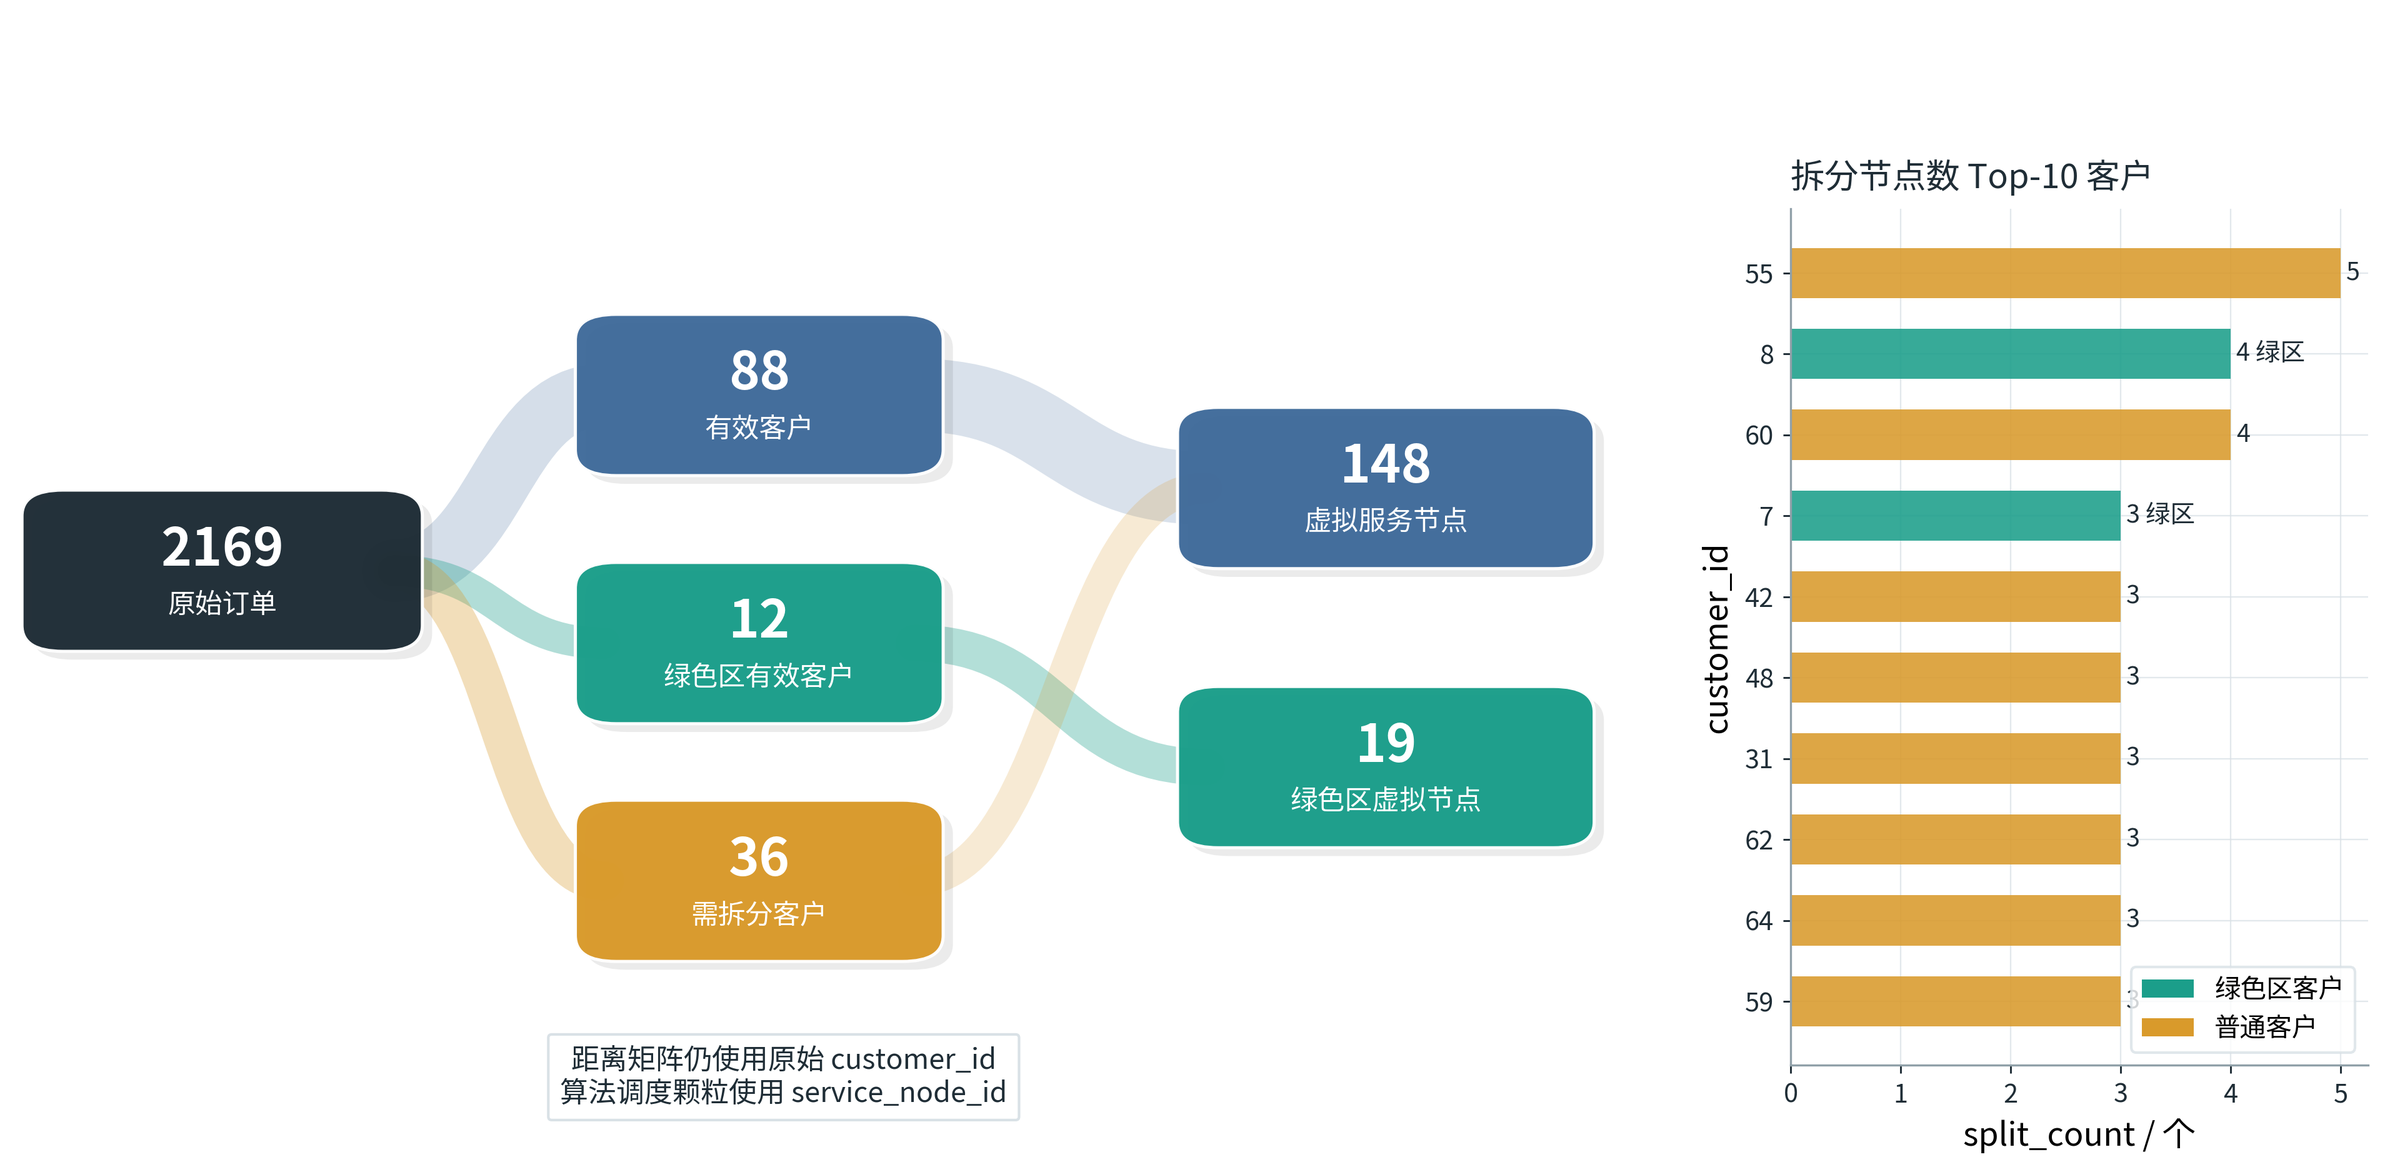
\includegraphics[width=0.95\textwidth]{fig01_order_aggregation_split_topology.png}
  \caption{订单聚合前后的拓扑流向图。图中展示 2169 条原始订单向 88 个有效客户和 148 个虚拟服务节点的转化关系，强调距离矩阵索引与算法服务颗粒的分离。}
  \label{fig:order-aggregation}
\end{figure}
\subsection{5.3 绿色配送区判定}

补充说明要求按坐标计算绿色配送区客户数量。设客户 \(c\) 坐标为 \((x_c,y_c)\)，绿色区指标为

\[
g_c=\mathbf{1}\{x_c^2+y_c^2\le 10^2\}.
\]

据此核算，有订单绿色区客户为 12 个，绿色区虚拟服务节点为 19 个。配送中心坐标为 \((20,20)\)，不在绿色区圆心处。后续所有绿色政策判定均使用 \(g_c\)，不使用配送中心到客户的路网距离替代空间坐标判定。

客户需求与绿色配送区的空间关系见图\ref{fig:spatial-density}。

\begin{figure}[H]
  \centering
  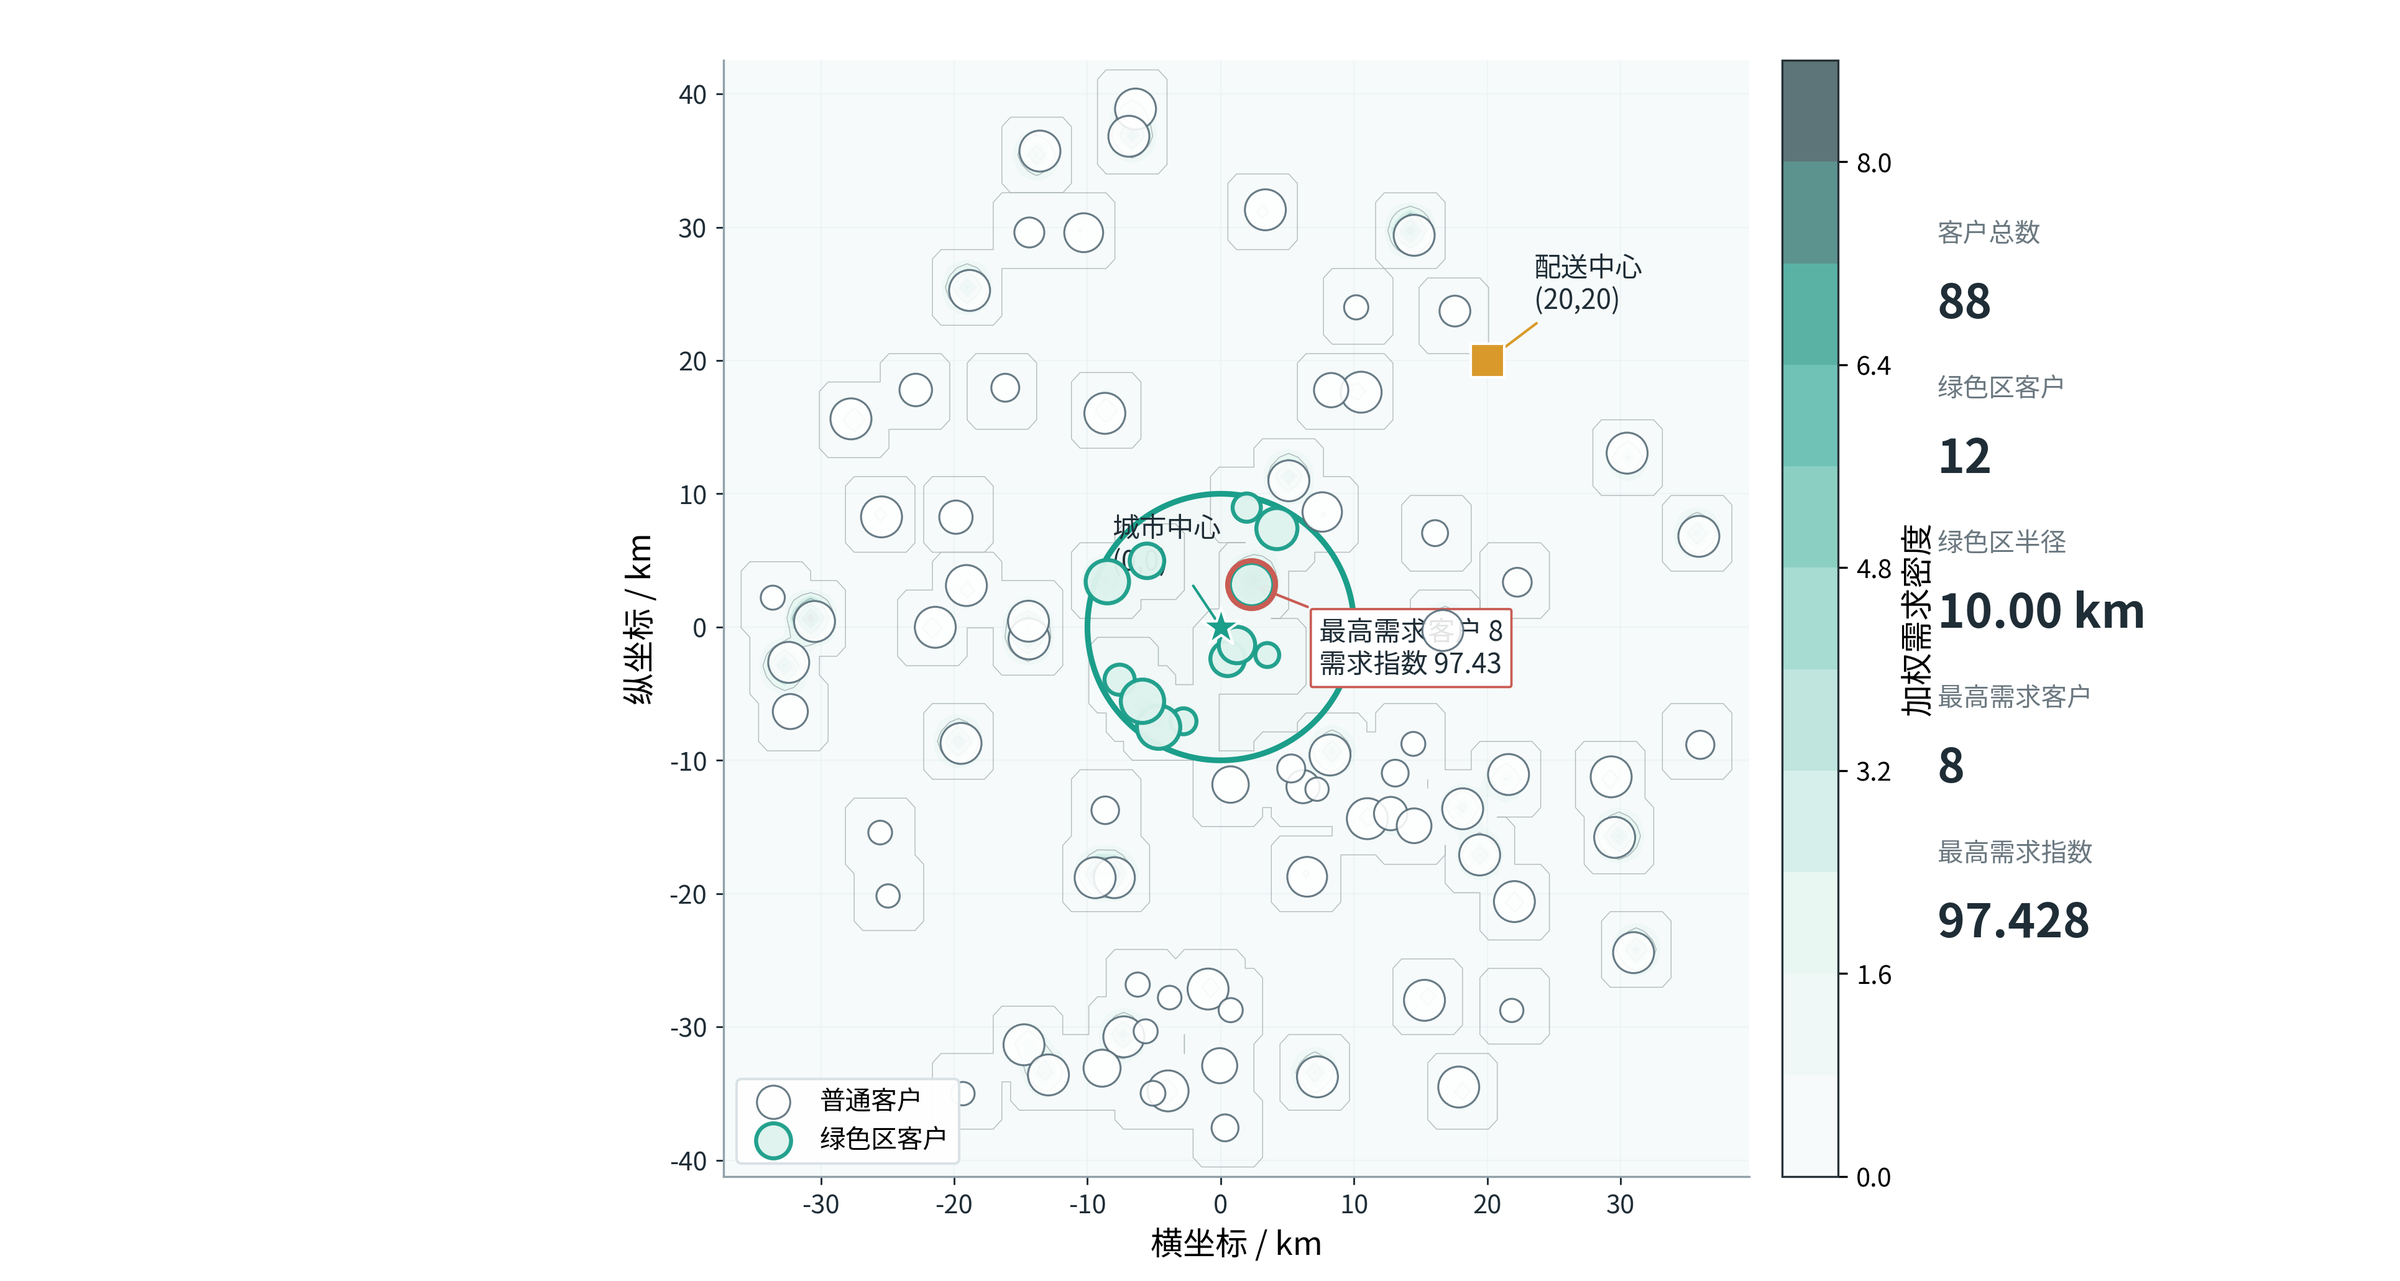
\includegraphics[width=0.95\textwidth]{fig02_customer_spatial_density.png}
  \caption{客户需求空间分布与绿色区约束。绿色配送区以城市中心 (0,0) 为圆心，配送中心位于 (20,20)，图中气泡和密度层仅表示客户需求分布。}
  \label{fig:spatial-density}
\end{figure}
\subsection{5.4 时间、距离与节点映射}

所有时间统一转化为从 0:00 起的绝对分钟数，8:00 为 480，16:00 为 960。题面时间窗最晚到 20:58，而补充说明只给出 17:00 前速度分布，因此本文将 17:00 后速度延拓为一般时段分布。

距离矩阵为原始节点间实际道路距离，索引是配送中心 0 和原始客户编号 1 至 98。虚拟服务节点不直接用于距离矩阵索引，任意虚拟节点 \(i,j\) 间距离写作 \(d_{c(i),c(j)}\)。这一区分贯穿成本计算、路线评价和政策检测。

\subsection{5.5 预处理质量控制}

预处理阶段直接决定后续模型是否可解释。本文对四类一致性进行检查：其一，聚合后的客户需求之和必须与 2169 条原始订单重量和体积总和一致；其二，拆分后的每个虚拟服务节点均不超过最大车辆的重量和体积容量，并继承原客户时间窗、坐标和绿色区标签；其三，任意距离查询必须先由 \texttt{service\_node\_id} 映射回原始 \texttt{customer\_id}，避免在距离矩阵中构造不存在的新行列；其四，绿色区判定只能由客户坐标到 \((0,0)\) 的欧氏距离给出，不能用配送中心 \((20,20)\) 或路网距离替代。上述检查使后续三问的成本差异能够追溯到路线、车型、时间和政策变化，而不是预处理口径变化。

从论文表达角度，预处理不仅是数据清洗，也是建模边界的第一次固定：订单聚合回答需求总量，虚拟拆分回答容量可行，绿色区判定回答政策对象，时间和节点映射回答算法可复现。后续表格均优先引用这些冻结后的基础事实，长订单明细和虚拟节点映射表放入支撑材料。


\section{六、模型建立与求解}

\subsection{6.1 公共时变异构车队配送模型}

三问共用相同的官方成本函数：

\[
\min C=C_{\mathrm{fixed}}+C_{\mathrm{energy}}+C_{\mathrm{carbon}}+C_{\mathrm{tw}}.
\]

其中固定成本按启用物理车辆计：

\[
C_{\mathrm{fixed}}=400\sum_{m}u_m.
\]

软时间窗定义为

\[
W_i=\max(e_i-a_i,0),\qquad L_i=\max(a_i-l_i,0),
\]

\[
C_{\mathrm{tw}}=\sum_{i\in S}\left(\frac{20}{60}W_i+\frac{50}{60}L_i\right).
\]

若车辆到达早于时间窗下界，则开始服务时刻为

\[
b_i=\max(a_i,e_i),
\]

离开时刻为 \(b_i+20\)。

\subsubsection{6.1.1 时变行驶时间}

补充说明给出的速度分布如下。

\begin{table}[H]
\centering
\small
\caption{时变速度参数}
\label{tab:speed-periods}
\begin{tabularx}{\textwidth}{>{\raggedright\arraybackslash}X>{\raggedright\arraybackslash}X>{\raggedright\arraybackslash}X>{\raggedright\arraybackslash}X}
\toprule
时段 & 时间范围 & 均值 \(\mu\)/(km/h) & 标准差 \(\sigma\)/(km/h) \\
\midrule
拥堵 & 8:00-9:00，11:30-13:00 & 9.8 & 4.7 \\
顺畅 & 9:00-10:00，13:00-15:00 & 55.3 & 0.1 \\
一般 & 10:00-11:30，15:00-17:00 & 35.4 & 5.2 \\
一般延拓 & 17:00 之后 & 35.4 & 5.2 \\
\bottomrule
\end{tabularx}
\end{table}

对路段 \((a,b)\)，若车辆在时刻 \(t\) 出发，行驶过程可能跨越多个速度时段。本文按时段分段积分，设跨越子段集合为 \(P_{ab}(t)\)，每段距离为 \(\Delta d_p\)，则行驶时间为

\[
\tau_{ab}(t)=\sum_{p\in P_{ab}(t)}\frac{60\Delta d_p}{\mu_p}.
\]

路线上的到达时间递推为

\[
a_j=t_i+\tau_{c(i),c(j)}(t_i),
\]

其中 \(t_i\) 为离开上一节点的时刻。分段积分避免跨越速度时段边界时使用单一出发时刻速度造成的时间误差。

上述分段速度、二阶矩修正与载重率之间的作用关系见图\ref{fig:speed-energy-mechanism}；随后图\ref{fig:speed-energy} 给出由 CSV 直接生成的定量能耗曲面。

\begin{figure}[H]
  \centering
  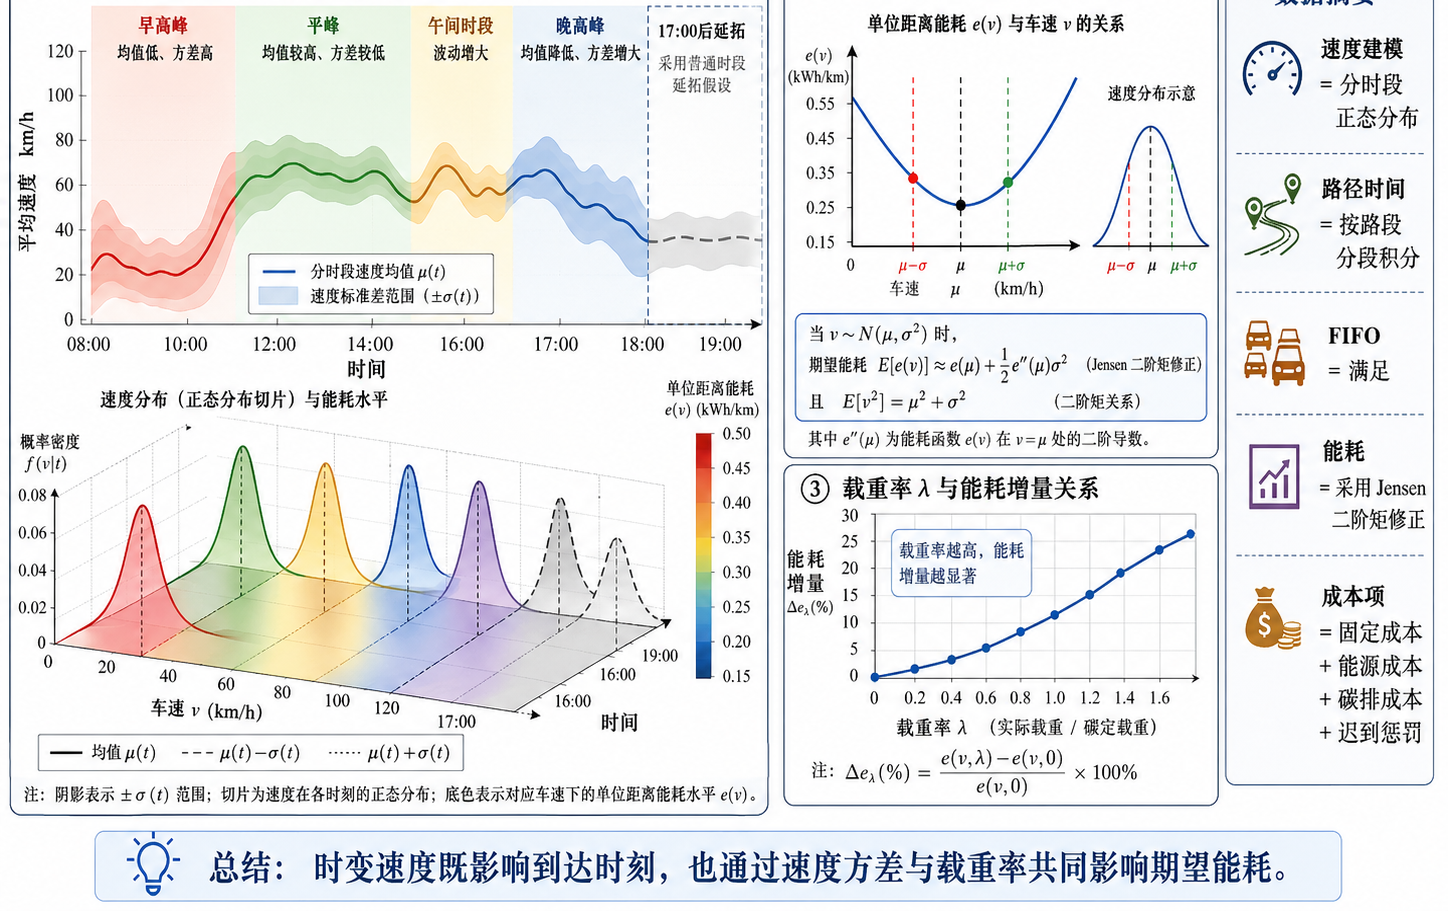
\includegraphics[width=0.92\textwidth]{fig03a_speed_energy_mechanism.png}
  \caption{时变速度--时间--能耗关系机制示意。该图用于解释分时段速度、Jensen 二阶矩修正和载重率对能耗估计的耦合关系；定量结果以题面函数和图\ref{fig:speed-energy} 的 CSV 曲面为准。}
  \label{fig:speed-energy-mechanism}
\end{figure}

\subsubsection{6.1.2 载重相关能耗与碳排}

题面给出燃油车和新能源车能耗函数分别为

\[
g_F(v)=0.0025v^2-0.2554v+31.75,
\]

\[
g_E(v)=0.0014v^2-0.12v+36.19.
\]

由于速度为随机变量且能耗含二次项，本文采用

\[
E[v^2]=\mu^2+\sigma^2
\]

计算期望能耗：

\[
E[g_F(v_p)]=0.0025(\mu_p^2+\sigma_p^2)-0.2554\mu_p+31.75,
\]

\[
E[g_E(v_p)]=0.0014(\mu_p^2+\sigma_p^2)-0.12\mu_p+36.19.
\]

设车辆进入某弧段前的剩余载重为 \(w\)，车型 \(k\) 的载重上限为 \(Q_k\)，载重率为

\[
\rho=\frac{w}{Q_k}.
\]

本文在路线评价中，对每段弧 \((a,b)\) 使用车辆离开节点 \(a\) 时的实时载重 \(w\)，即 \(\rho\) 随沿途卸货而递减，体现配送过程中能耗随载重降低的变化。

燃油车和新能源车的载重修正系数分别取 \(1+0.40\rho\) 与 \(1+0.35\rho\)。跨时段弧段的燃油消耗和电耗为

\[
E^F_{ab}=(1+0.40\rho)\sum_{p\in P_{ab}(t)}\frac{\Delta d_p}{100}E[g_F(v_p)],
\]

\[
E^E_{ab}=(1+0.35\rho)\sum_{p\in P_{ab}(t)}\frac{\Delta d_p}{100}E[g_E(v_p)].
\]

能源成本为

\[
C_{\mathrm{energy}}=7.61\sum E^F_{ab}+1.64\sum E^E_{ab}.
\]

燃油碳排因子为 \(2.547\) kg/L，电力碳排因子为 \(0.501\) kg/kWh，碳价为 \(0.65\) 元/kg，故

\[
G=2.547\sum E^F_{ab}+0.501\sum E^E_{ab},
\]

\[
C_{\mathrm{carbon}}=0.65G.
\]

速度时段、载重率与单位能耗的耦合关系见图\ref{fig:speed-energy}。

\begin{figure}[H]
  \centering
  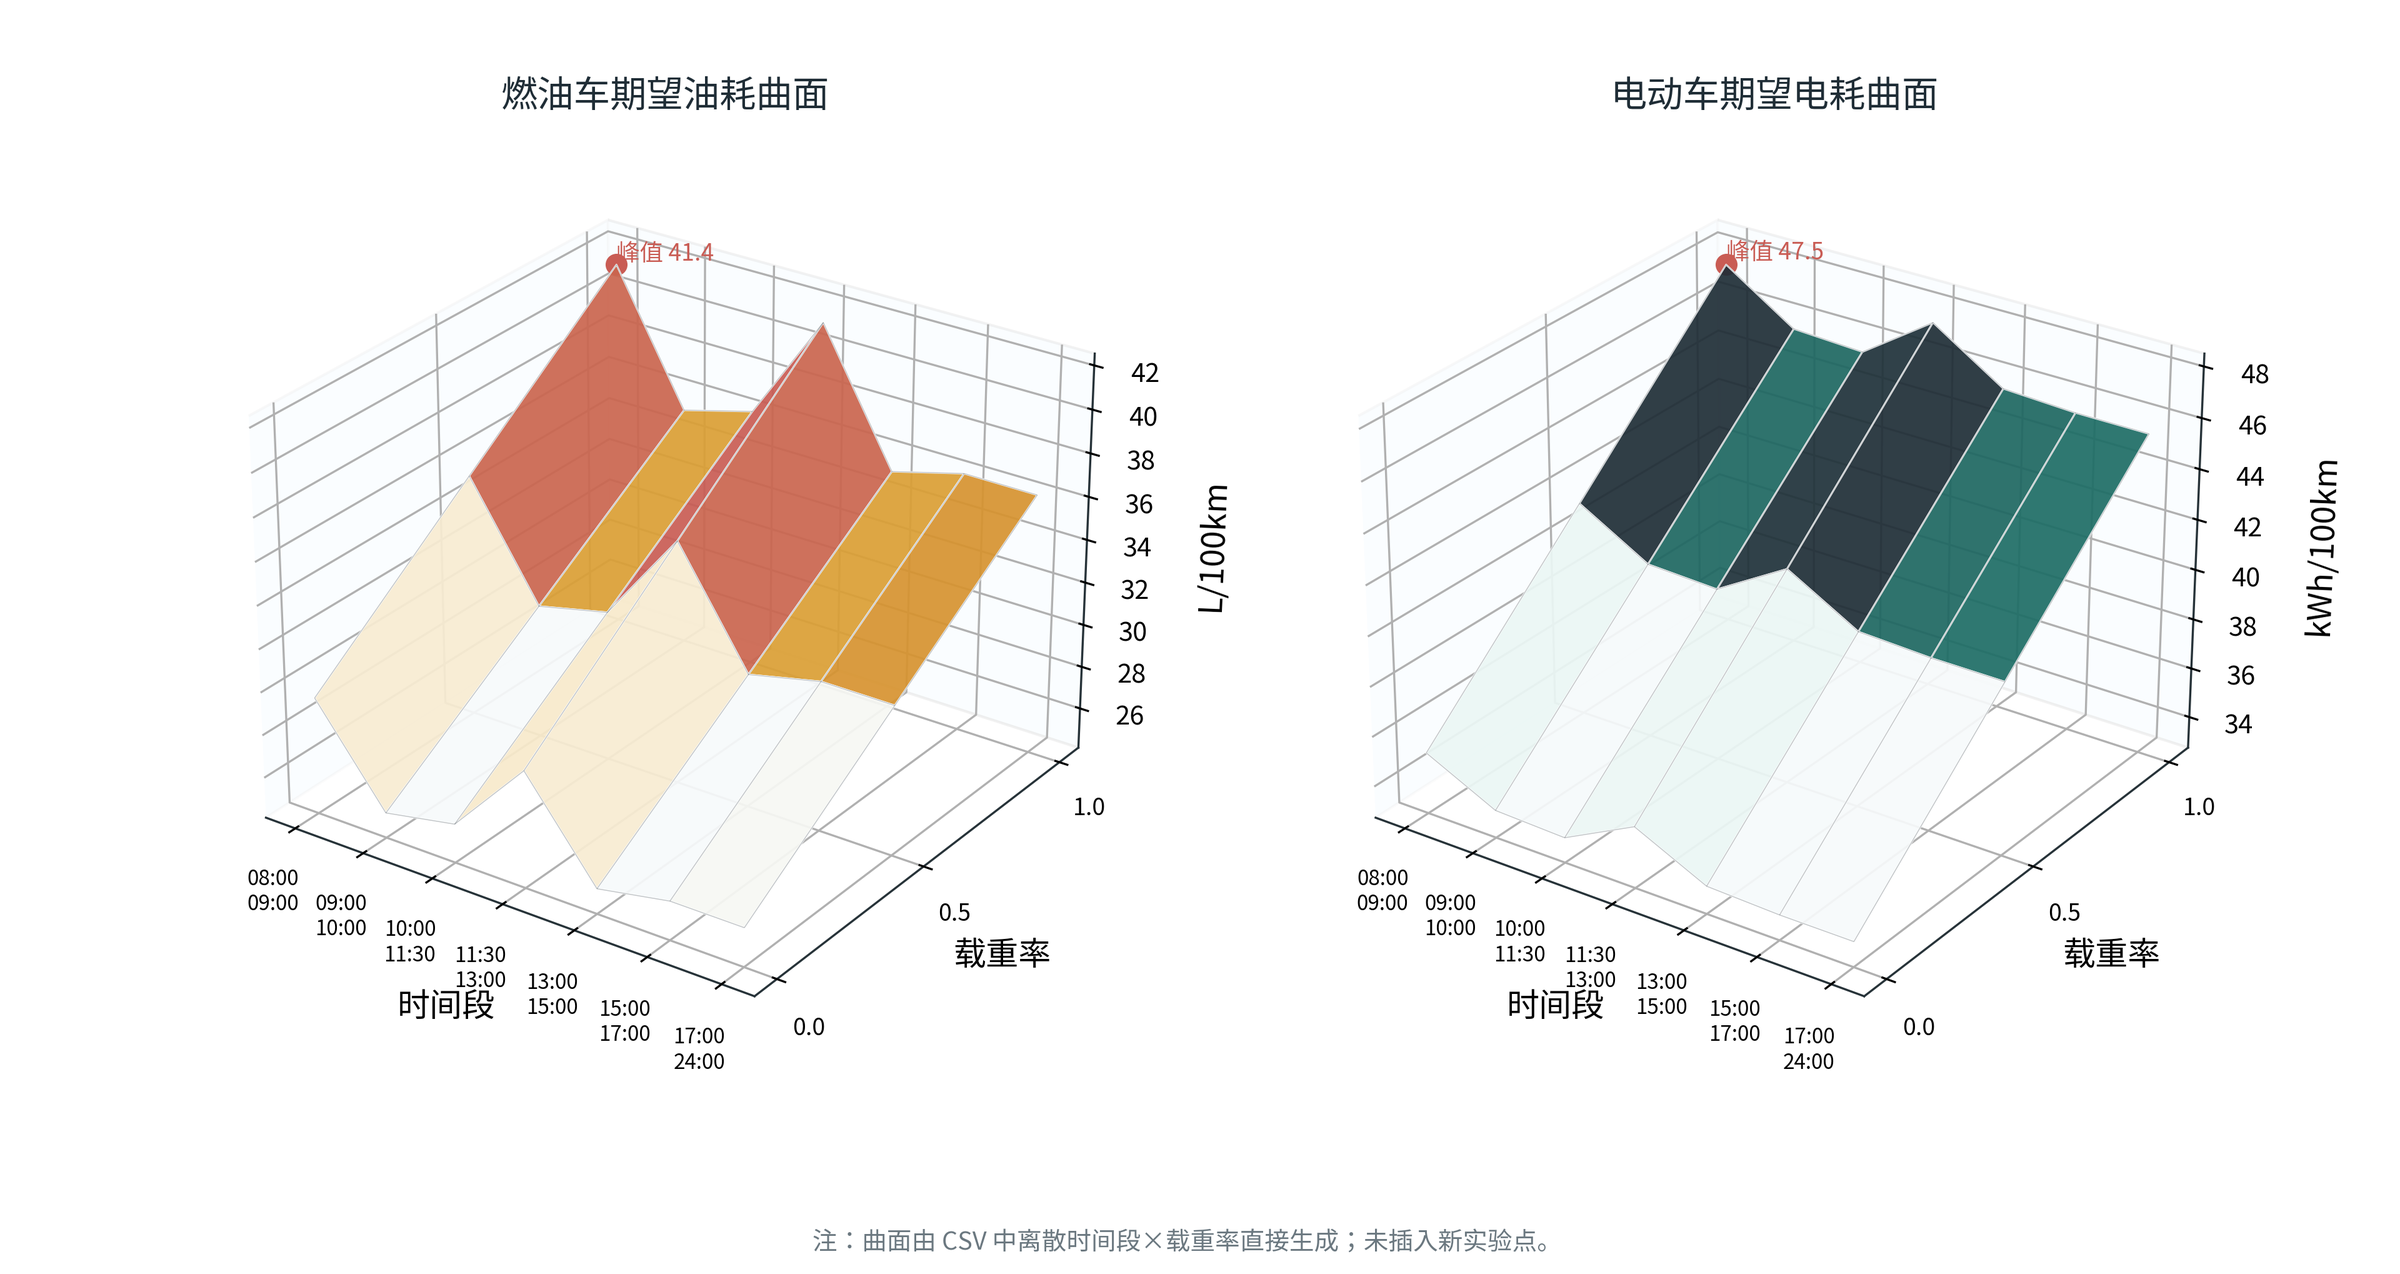
\includegraphics[width=0.95\textwidth]{fig03_speed_energy_surface.png}
  \caption{时变速度与载重率耦合下的单位能耗曲面。燃油车与电动车均按题面能耗函数计算，电动车电耗后续仍计入电力碳排。}
  \label{fig:speed-energy}
\end{figure}
\subsubsection{6.1.3 基础约束}

覆盖约束为

\[
\sum_{r\in R}\sum_{j\in S\cup\{0\}}x_{ijr}=1,\qquad \forall i\in S.
\]

容量约束为

\[
\sum_{i\in r}q_i\le Q_k,\qquad \sum_{i\in r}v_i\le V_k,\qquad \forall r,k.
\]

物理车辆数量约束为

\[
\sum_{m\in M_k}u_m\le |M_k|,\qquad \forall k\in K.
\]

同一物理车辆执行连续趟次时满足时间链约束：

\[
T_{r_2}\ge \mathrm{return}_{r_1},
\]

其中 \(r_2\) 是同一车辆在 \(r_1\) 之后执行的趟次。

\subsection{6.2 第一问：静态调度模型与求解}

\subsubsection{6.2.1 建模思路}

第一问不考虑绿色限行政策，目标是在全部服务节点覆盖和容量可行的前提下最小化官方总成本。本文把虚拟服务节点视为最小服务单元，每条路线表示一次 depot-to-depot 趟次。求解时先构造容量合法的趟次，再将趟次分配给物理车辆，最后通过 ALNS 对节点顺序和趟次组合进行改进。

变量说明如下：\(x_{ijr}\) 描述趟次 \(r\) 是否从节点 \(i\) 直接到节点 \(j\)，用于刻画路线访问顺序；\(y_{rk}\) 描述趟次车型，决定容量、能耗函数和车辆类型；\(u_m\) 描述物理车辆是否启用，用于计算固定成本；\(a_i,W_i,L_i\) 分别表示到达、等待和迟到，用于软时间窗成本；\(\rho_{ijr}\) 表示弧段行驶前载重率，用于载重相关能耗。上述变量服务于三个目标：保证所有虚拟节点被服务，递推出时变到达时间，计算载重相关能耗与碳排。

\subsubsection{6.2.2 算法流程}

第一问采用“初始解构造 + 物理车辆排班 + ALNS 优化 + 诊断修正”的启发式框架。

\begin{enumerate}[leftmargin=2em,itemsep=0.2em]
\item 读取预处理后的客户需求、虚拟服务节点、坐标、距离矩阵和时间窗。
\item 按时间窗中心、需求规模和容量压力排序服务节点。
\item 贪心构造容量合法的 depot-to-depot 趟次。
\item 将趟次分配给同车型物理车辆，保证物理车辆连续趟次时间链可行。
\item 使用 ALNS 迭代执行破坏和修复：随机删除、高成本删除、相关节点删除、时间窗罚金删除、迟到后缀删除等破坏算子，配合贪心插入、Regret 插入和时间导向插入。
\item 对每个候选解完整重算官方成本和服务质量指标。
\item 以官方总成本为正式选择标准，服务质量指标仅用于诊断。
\end{enumerate}

算法设计的可解释性体现在两点。首先，破坏算子分别对应成本高、空间相关、时间窗紧张和迟到后缀等业务诱因，使搜索能够针对题面中的主要冲突来源进行局部重排。其次，每次插入后都重新递推到达时间、载重率、能耗、碳排和软时间窗罚金，避免只用距离增量近似评价候选路线。该流程虽然属于启发式搜索，但每个候选解都经过完整成本重构和硬约束检查，便于在论文中复核。

第一问正式结果见表\ref{tab:p1-result}。

\begin{table}[H]
\centering
\small
\caption{第一问正式调度结果}
\label{tab:p1-result}
\begin{tabularx}{\textwidth}{>{\raggedright\arraybackslash}X>{\raggedright\arraybackslash}X}
\toprule
指标 & 数值 \\
\midrule
总成本/元 & 48644.68 \\
固定成本/元 & 17200.00 \\
能源成本/元 & 25091.79 \\
碳排成本/元 & 5419.37 \\
软时间窗罚金/元 & 933.53 \\
总行驶距离/km & 13384.29 \\
碳排放/kg & 8337.49 \\
depot-to-depot 趟次数 & 116 \\
启用物理车辆 & E1:10, F1:33 \\
趟次使用 & E1:32, F1:84 \\
迟到点 / 最大迟到 & 4 / 31.60 min \\
覆盖与容量 & 可行 \\
\bottomrule
\end{tabularx}
\end{table}

第一问静态调度的空间覆盖与迟到风险见图\ref{fig:p1-route-risk}。

\begin{figure}[H]
  \centering
  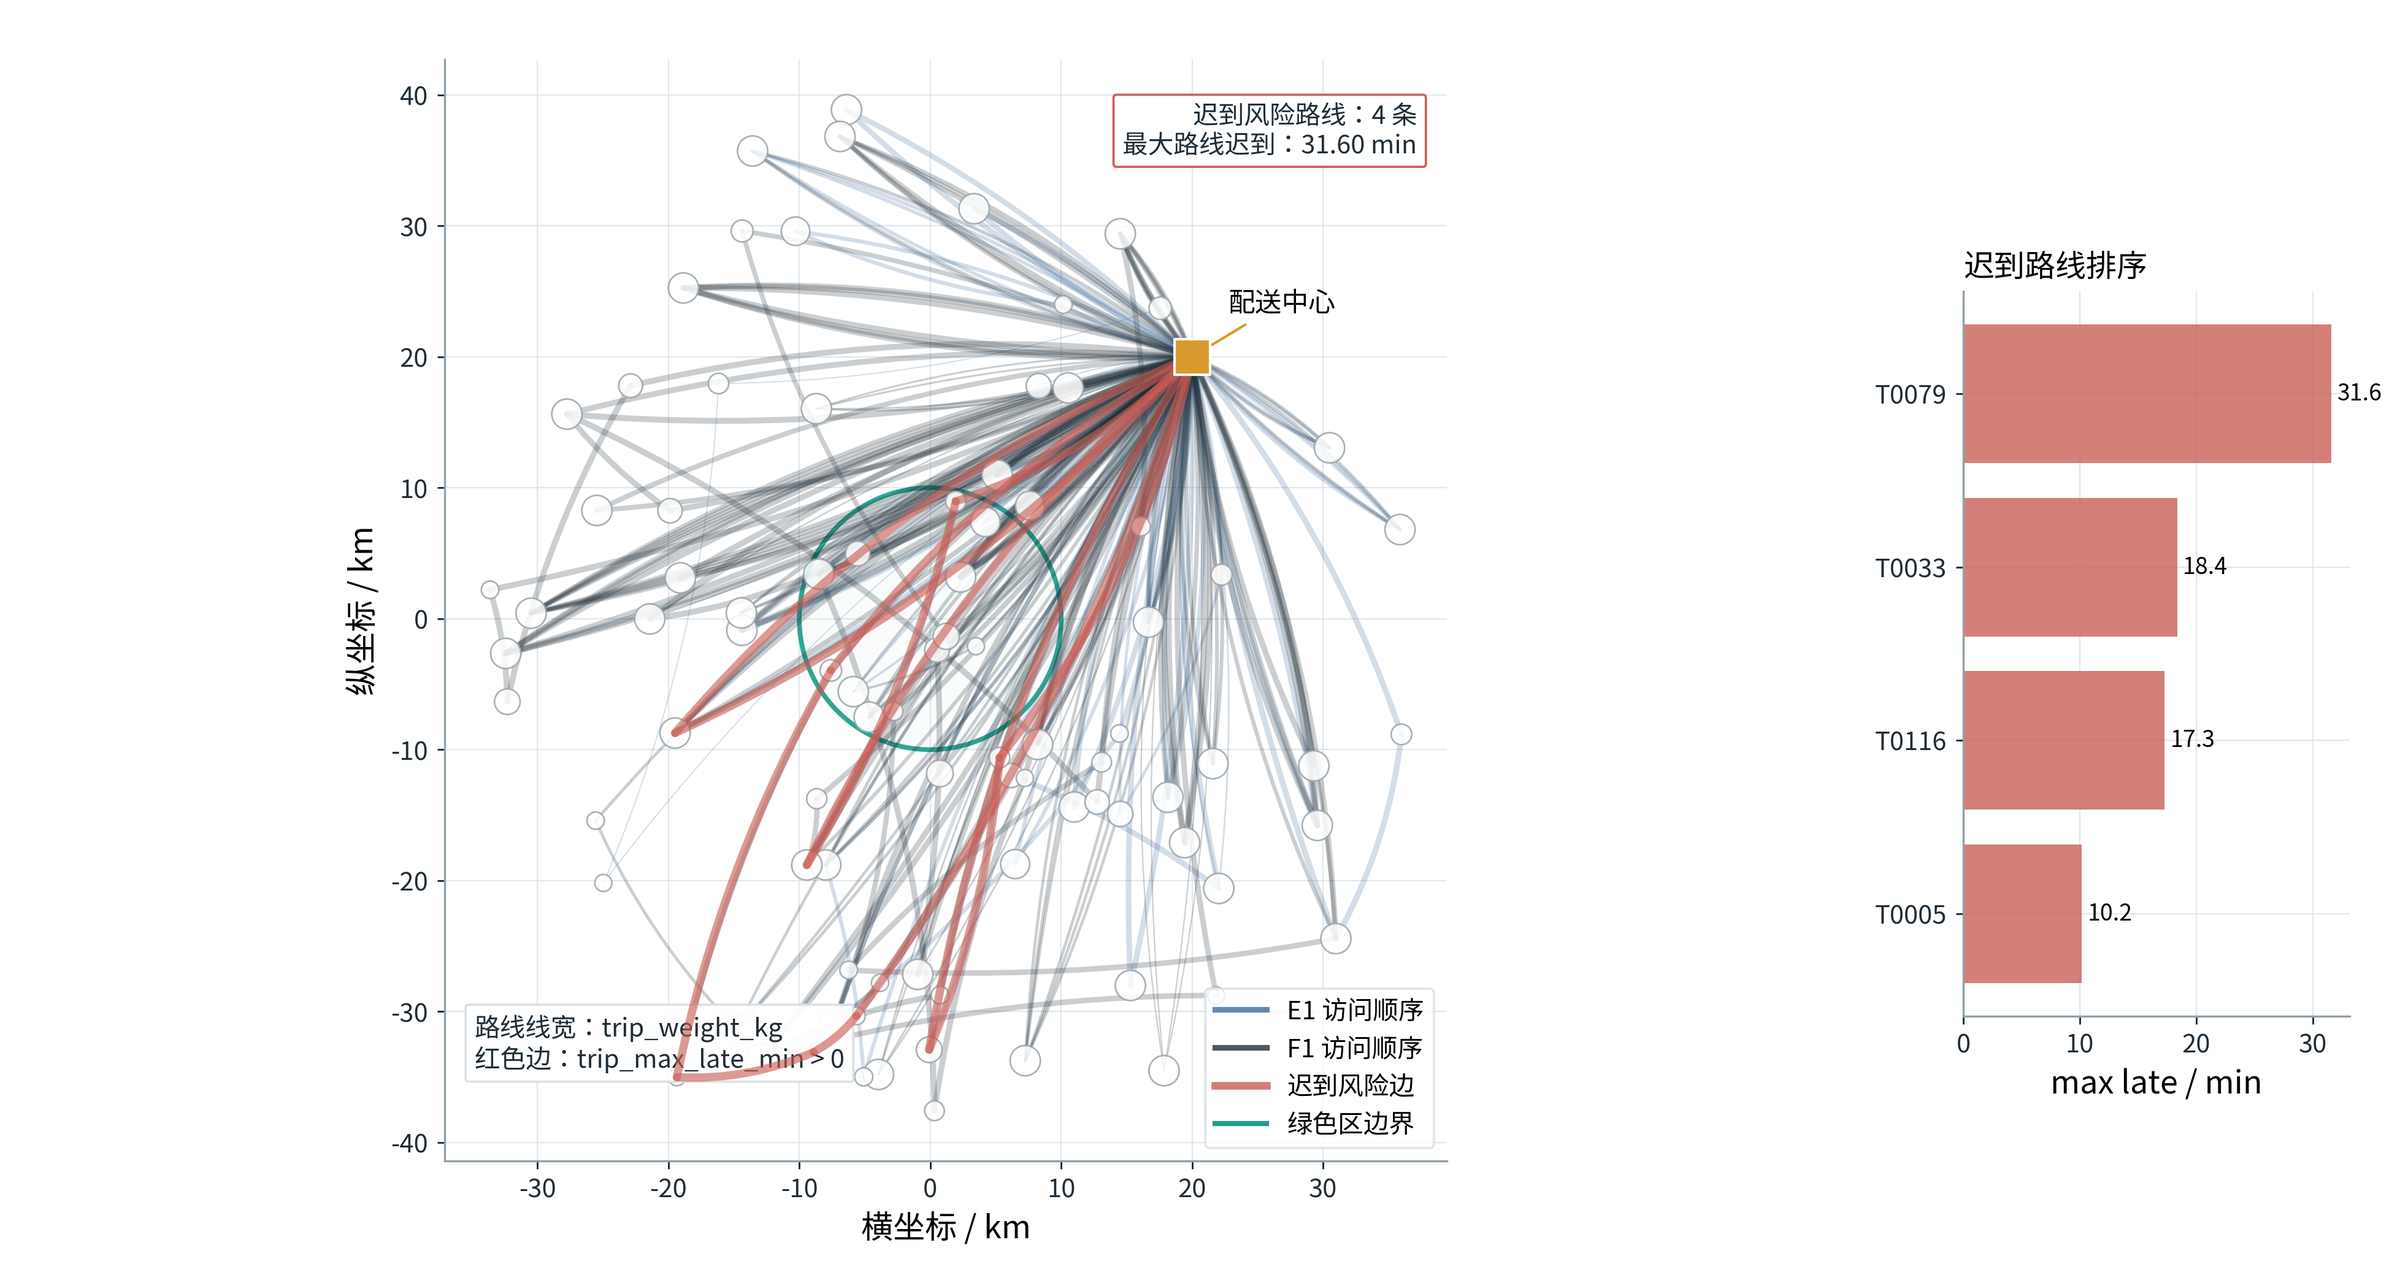
\includegraphics[width=0.95\textwidth]{fig04_problem1_route_risk_bundle.png}
  \caption{第一问静态调度路线束与迟到风险。折线仅表示访问顺序，不代表真实道路轨迹；红色描边表示存在迟到风险的趟次。}
  \label{fig:p1-route-risk}
\end{figure}
\subsubsection{6.2.3 结果解释}

第一问能源成本占总成本比例最高，约为 \texttt{51.58\%}；固定成本约占 \texttt{35.36\%}，碳排成本约占 \texttt{11.14\%}，软时间窗罚金约占 \texttt{1.92\%}。该结构说明，在本题给定路网距离和大批量需求下，路径长度、速度时段和载重状态共同决定主要成本，而时间窗主要通过少量迟到点进行边际调节。正式方案只使用 E1 和 F1 两类大车，表明在大量虚拟节点重量较高的条件下，高载重车辆可以减少小车带来的趟次扩张和排班复杂度。

4 个迟到点不破坏可行性，因为题目时间窗为软约束。根据迟到诊断，残余迟到分别来自直达也迟到、多趟物理车辆级联和局部路线顺序问题。进一步追求零迟到可能降低服务风险，但会改变成本-服务质量权衡，因此第一问正式结果仍按官方总成本选择。

\subsubsection{6.2.4 局限说明}

第一问使用启发式搜索，不能给出全局最优证明；题面没有给出 17:00 后速度分布，晚间行驶时间和能耗依赖延拓假设；模型未显式考虑装卸重装时间、车辆维护和司机工时等运营细节。上述因素不影响本问的题面约束可行性，但应作为模型改进方向保留。

\subsection{6.3 第二问：绿色限行硬约束模型与求解}

\subsubsection{6.3.1 建模思路}

第二问在公共模型基础上加入绿色配送区限行约束。设 \(green(i)=1\) 表示虚拟服务节点 \(i\) 对应客户在绿色区，\(fuel(k)=1\) 表示车型 \(k\) 为燃油车。限行窗口为 \([480,960)\)，则硬约束为

\[
fuel(k)\land green(i)\land 480\le a_i<960 \Rightarrow \text{infeasible}.
\]

在论文表述中，也可写作

\[
c(i)\in G,\ k(r)\in K_F \Rightarrow a_i\notin[480,960).
\]

变量说明如下：\(green(i)\) 为服务节点 \(i\) 的绿色区指示变量，由 \(c(i)\) 的坐标计算；\(fuel(k)\) 为车型 \(k\) 的燃油车指示变量；\(a_i\) 为节点到达时刻，是判断限行窗口的时间变量；\(p_i\) 可作为政策冲突诊断变量，但正式可行解要求 \(\sum_i p_i=0\)。该约束是正式可行性条件，不是成本项。本文在搜索中可使用 EV reservation 作为调度评分辅助，使稀缺 E1 更倾向于服务受政策影响的绿色区任务；但最终成本仍按四项官方成本计算，EV reservation 不进入结果表中的总成本。

绿色限行的空间围栏与时间禁行窗口可抽象为图\ref{fig:green-constraint-mechanism} 所示的时空双重可行域。

\begin{figure}[H]
  \centering
  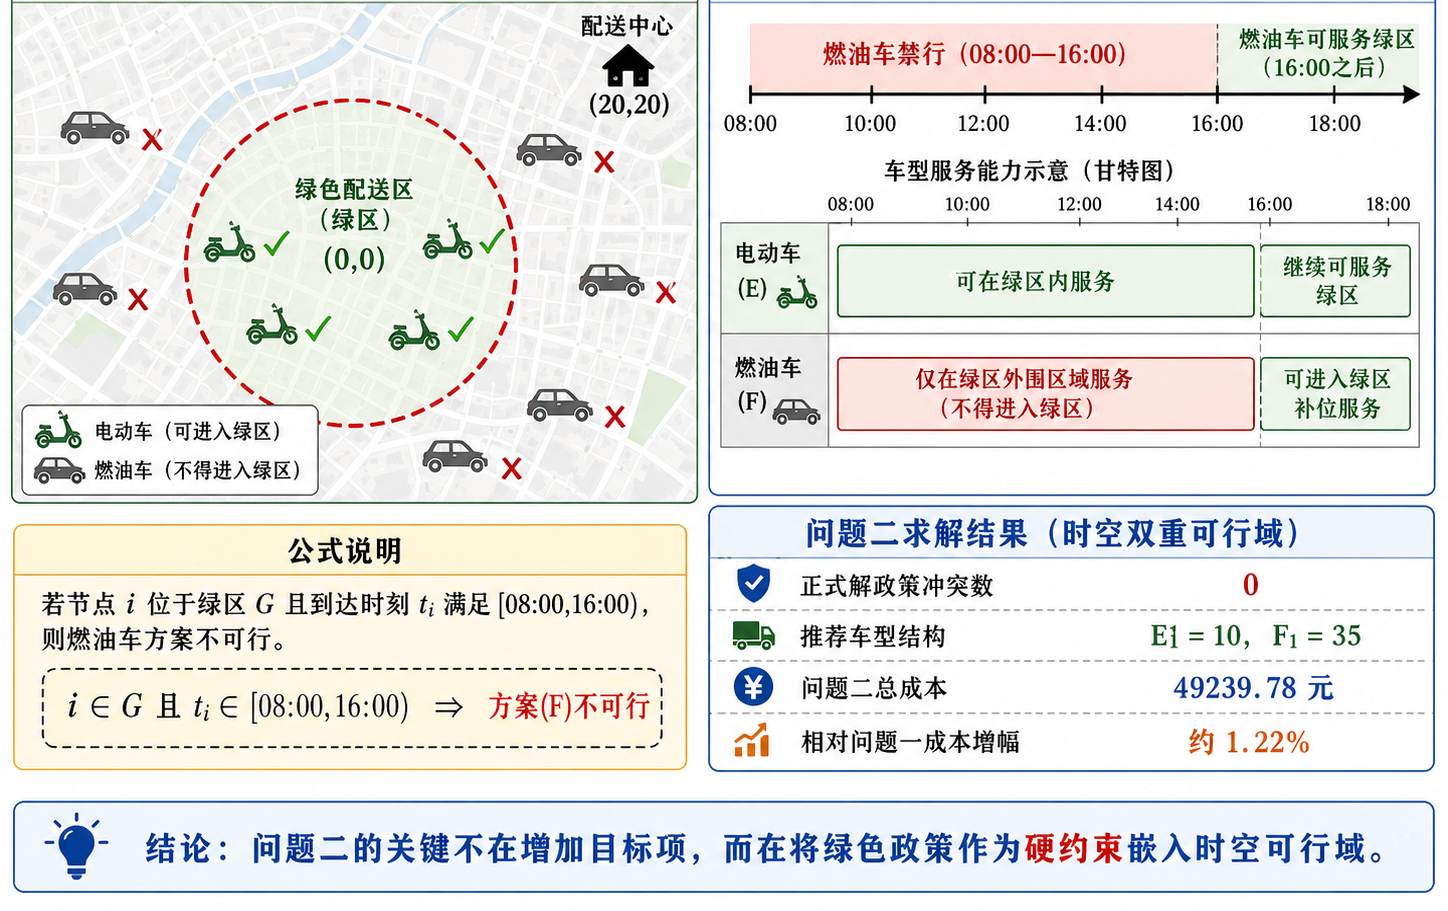
\includegraphics[width=0.92\textwidth]{fig06a_green_constraint_mechanism.png}
  \caption{绿色约束的时空双重可行域示意。图中车辆图标仅用于说明绿色区服务事件的车型--时段可行性，不表示道路几何轨迹或路段穿越检测。}
  \label{fig:green-constraint-mechanism}
\end{figure}

\subsubsection{6.3.2 候选方案与算法流程}

第二问比较三类服务节点方案：

\begin{enumerate}[leftmargin=2em,itemsep=0.2em]
\item \texttt{DEFAULT\_SPLIT}：沿用第一问默认拆分，服务节点数为 148。
\item \texttt{GREEN\_HOTSPOT\_PARTIAL}：只对部分绿色区高风险客户做局部细拆，服务节点数为 153。
\item \texttt{GREEN\_E2\_ADAPTIVE}：按 E2 容量对绿色区客户做更细拆分，服务节点数为 166。
\end{enumerate}

求解流程为：

\begin{enumerate}[leftmargin=2em,itemsep=0.2em]
\item 读取指定拆分变体下的服务节点集合。
\item 构造初始趟次，并优先识别绿色区服务需求。
\item 在 ALNS 修复阶段过滤违反绿色限行硬约束的插入。
\item 在排班阶段检查物理车辆时间链和政策冲突。
\item 对完整、容量可行且政策冲突为 0 的候选解，按官方总成本排序。
\item 输出正式推荐方案和服务质量对照方案。
\end{enumerate}

与第一问相比，第二问求解的关键不是单纯增加车辆或改用新能源车，而是在绿色区客户、限行时段和车型属性之间重新分配稀缺服务能力。本文在搜索中把政策冲突作为硬过滤，使任何燃油车限行时段服务绿色区客户的插入立即被拒绝；同时把 EV reservation 仅作为搜索评分中的机会成本，用于提醒算法保留 E1 服务绿色区节点的能力。这样既能提升搜索效率，又不改变题面官方成本口径。

候选方案比较见表\ref{tab:p2-candidates}。

\begin{table}[H]
\centering
\small
\caption{第二问候选方案比较}
\label{tab:p2-candidates}
\begin{tabularx}{\textwidth}{>{\raggedright\arraybackslash}X>{\raggedright\arraybackslash}X>{\raggedright\arraybackslash}X>{\raggedright\arraybackslash}X>{\raggedright\arraybackslash}X>{\raggedright\arraybackslash}X>{\raggedright\arraybackslash}X>{\raggedright\arraybackslash}X}
\toprule
方案 & 服务节点 & 绿色区服务节点数 & 总成本/元 & 政策冲突 & 物理车辆 & 迟到点 & 最大迟到/min \\
\midrule
DEFAULT\_SPLIT & 148 & 19 & 49239.78 & 0 & E1:10, F1:35 & 12 & 129.44 \\
GREEN\_HOTSPOT\_PARTIAL & 153 & 24 & 52312.11 & 0 & E1:10, E2:1, F1:35 & 22 & 119.21 \\
GREEN\_E2\_ADAPTIVE & 166 & 37 & 57504.49 & 0 & E1:10, E2:3, F1:44 & 24 & 253.00 \\
\bottomrule
\end{tabularx}
\end{table}

注：绿色区原始有订单客户数均为 12 个；表中绿色区服务节点数差异仅来自不同拆分粒度，不影响实际服务客户数量。\texttt{GREEN\_E2\_ADAPTIVE} 的总成本以 \texttt{outputs/problem2/variant\_comparison.csv} 为准。

正式推荐 \texttt{DEFAULT\_SPLIT}，其成本分项见表\ref{tab:p2-result}。

\begin{table}[H]
\centering
\small
\caption{第二问正式推荐方案结果}
\label{tab:p2-result}
\begin{tabularx}{\textwidth}{>{\raggedright\arraybackslash}X>{\raggedright\arraybackslash}X}
\toprule
指标 & 数值 \\
\midrule
总成本/元 & 49239.78 \\
固定成本/元 & 18000.00 \\
能源成本/元 & 24551.90 \\
碳排成本/元 & 5301.72 \\
软时间窗罚金/元 & 1386.17 \\
总行驶距离/km & 13093.90 \\
碳排放/kg & 8156.49 \\
depot-to-depot 趟次数 & 115 \\
趟次使用 & E1:28, F1:87 \\
启用物理车辆 & E1:10, F1:35 \\
政策冲突 & 0 \\
覆盖与容量 & 可行 \\
迟到点 / 最大迟到 & 12 / 129.44 min \\
\bottomrule
\end{tabularx}
\end{table}

上述正式推荐方案以官方总成本最小为选择标准。为说明成本最小与准时性改善之间的可量化权衡，本文在 6.3.4 节保留服务质量对照方案，其成本为 \texttt{50770.72} 元，迟到点为 \texttt{2} 个，最大迟到为 \texttt{5.93 min}，仅供管理者按业务优先级参考。

绿色限行政策对成本、碳排和车队结构的影响见图\ref{fig:policy-shift}。

\begin{figure}[H]
  \centering
  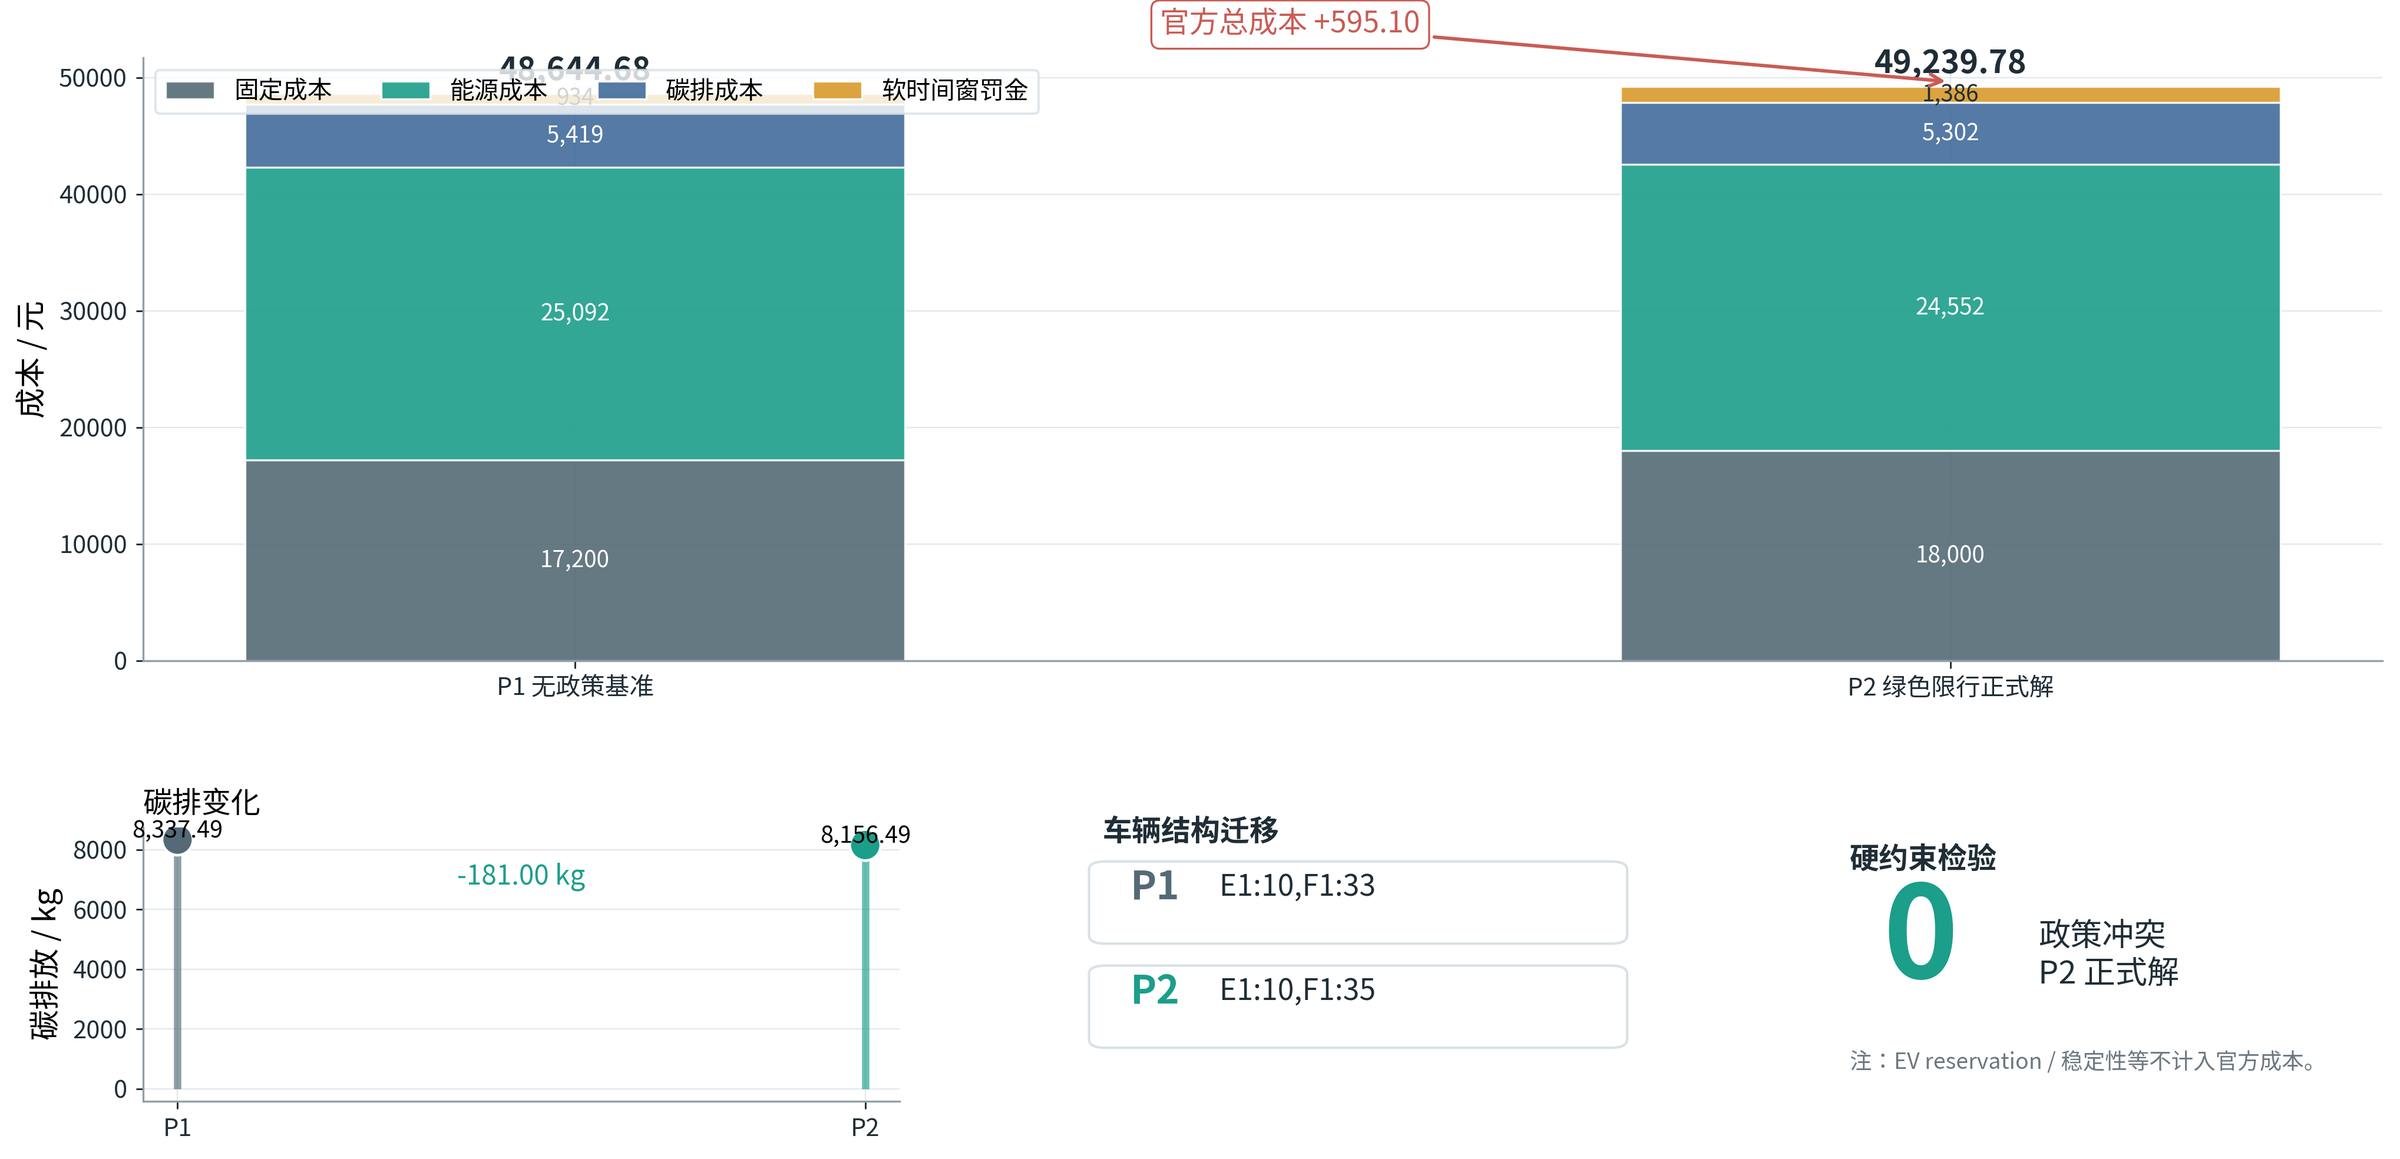
\includegraphics[width=0.96\textwidth]{fig05_policy_cost_carbon_fleet_shift.png}
  \caption{绿色限行政策前后的成本、碳排与车队结构迁移。成本堆叠仅包含固定成本、能源成本、碳排成本和软时间窗罚金。}
  \label{fig:policy-shift}
\end{figure}
绿色区服务时刻与车型合规性见图\ref{fig:green-policy-timeline}。

\begin{figure}[H]
  \centering
  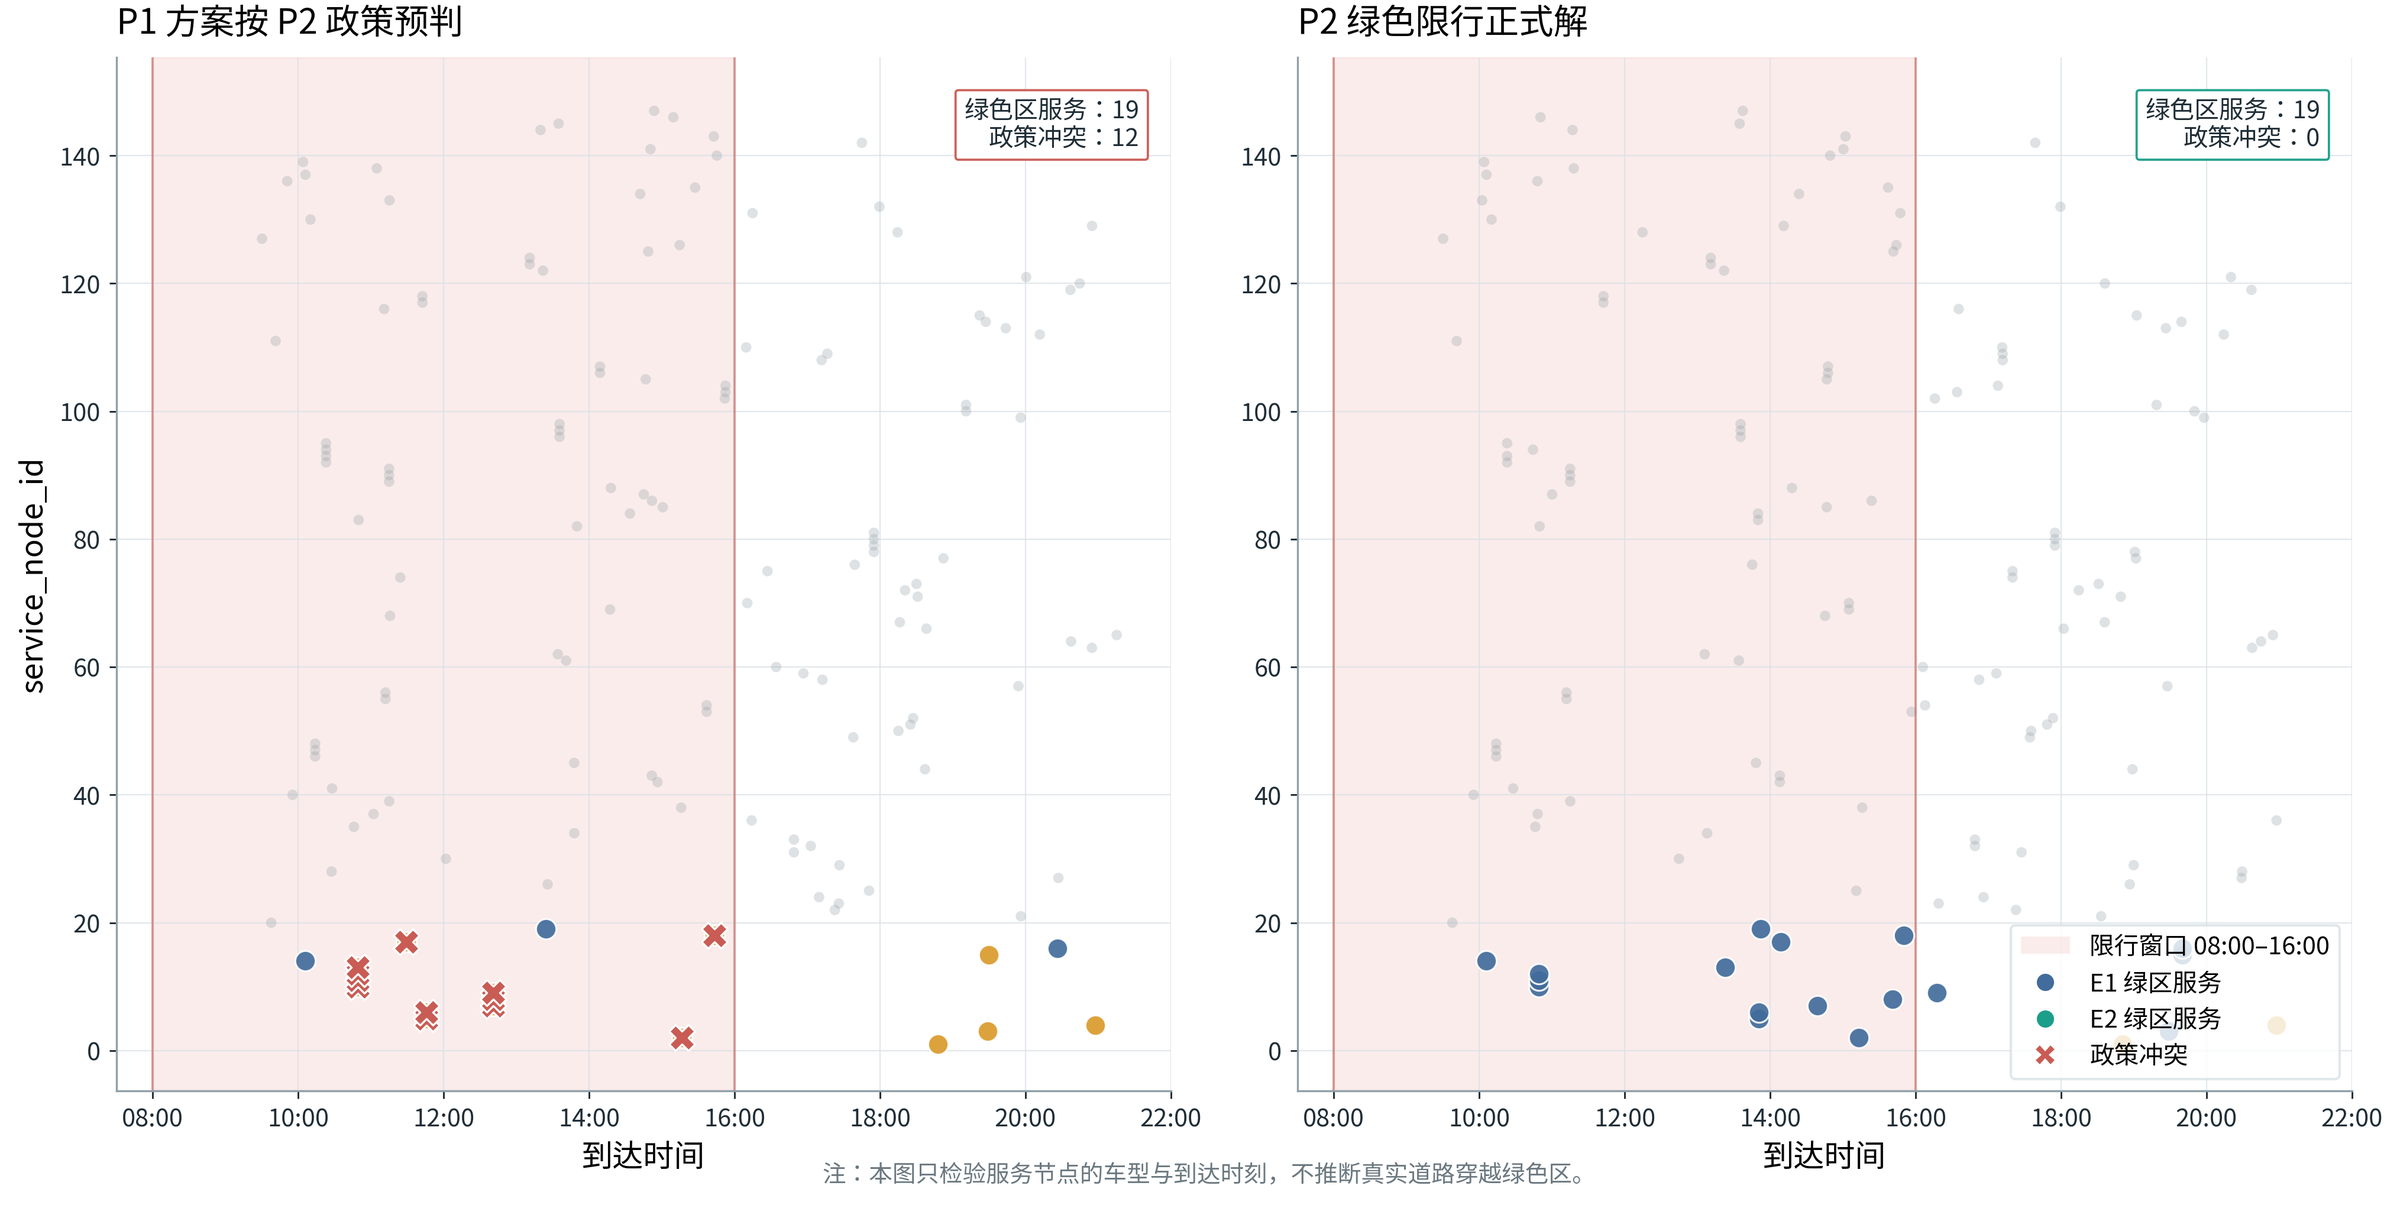
\includegraphics[width=0.95\textwidth]{fig06_green_zone_service_policy_timeline.png}
  \caption{绿色配送区服务时刻与车型合规检验。图中只检验绿色区客户服务事件，不推断道路几何穿越情况。}
  \label{fig:green-policy-timeline}
\end{figure}
\subsubsection{6.3.3 与第一问比较}

第二问相对第一问总成本增加

\[
49239.78-48644.68=595.10.
\]

成本分项变化见表\ref{tab:p1-p2-cost-delta}。

\begin{table}[H]
\centering
\small
\caption{第一问与第二问成本分项变化}
\label{tab:p1-p2-cost-delta}
\begin{tabularx}{\textwidth}{>{\raggedright\arraybackslash}X>{\raggedright\arraybackslash}X>{\raggedright\arraybackslash}X>{\raggedright\arraybackslash}X}
\toprule
成本项 & 第一问/元 & 第二问/元 & 变化/元 \\
\midrule
固定成本 & 17200.00 & 18000.00 & +800.00 \\
能源成本 & 25091.79 & 24551.90 & -539.89 \\
碳排成本 & 5419.37 & 5301.72 & -117.65 \\
软时间窗罚金 & 933.53 & 1386.17 & +452.64 \\
总成本 & 48644.68 & 49239.78 & +595.10 \\
\bottomrule
\end{tabularx}
\end{table}

该结果说明，绿色限行压缩了可行域，主要使固定成本和时间窗罚金上升；同时，重新组织路线降低了部分能源消耗和碳排成本。总成本上升幅度约为第一问成本的 \texttt{1.22\%}，可解释为政策合规的低幅成本代价。

从碳排角度看，第二问碳排量由第一问的 \texttt{8337.49 kg} 降至 \texttt{8156.49 kg}，减少约 \texttt{181.00 kg}。这说明绿色限行并非只带来成本上升：在硬合规约束下，路线重排和车型结构变化也带来了能源消耗与碳排分项的下降。本文因此将第二问结论表述为“低幅成本代价下实现政策硬合规，并伴随碳排分项改善”，而不把政策冲突写入成本。

\subsubsection{6.3.4 成本-服务质量权衡}

第二问正式推荐方案以官方总成本最低为选择标准，其最大迟到为 \texttt{129.44 min}，体现了成本优先目标下对软时间窗罚金的权衡。为刻画管理者可能关注的准时性目标，本文引用服务质量对照方案作为灵敏度分析，而非正式推荐。

\begin{table}[H]
\centering
\small
\caption{第二问服务质量对照方案}
\label{tab:p2-service-tradeoff}
\begin{tabularx}{\textwidth}{>{\raggedright\arraybackslash}X>{\raggedright\arraybackslash}X>{\raggedright\arraybackslash}X>{\raggedright\arraybackslash}X>{\raggedright\arraybackslash}X>{\raggedright\arraybackslash}X}
\toprule
方案 & 总成本/元 & 政策冲突 & 迟到点 & 最大迟到/min & 论文定位 \\
\midrule
DEFAULT\_SPLIT & 49239.78 & 0 & 12 & 129.44 & 正式成本推荐 \\
POLICY\_OPS + EV\_RESERVATION\_P500 & 50770.72 & 0 & 2 & 5.93 & 服务质量对照 \\
\bottomrule
\end{tabularx}
\end{table}

服务质量对照方案将最大迟到降至 \texttt{5.93 min}，迟到点从 12 个降至 2 个，但总成本增加至 \texttt{50770.72} 元，比正式推荐高 \texttt{1530.94} 元。该对比说明，若管理者希望显著降低迟到风险，需要接受更高车辆调度成本；若以题面官方成本为主目标，则 \texttt{DEFAULT\_SPLIT} 是当前正式推荐。本文主动给出该 Pareto 对照，能够避免只报告单一最低成本解而忽略服务质量边界。

第二问候选方案的成本与准时性权衡见图\ref{fig:p2-pareto}。

\begin{figure}[H]
  \centering
  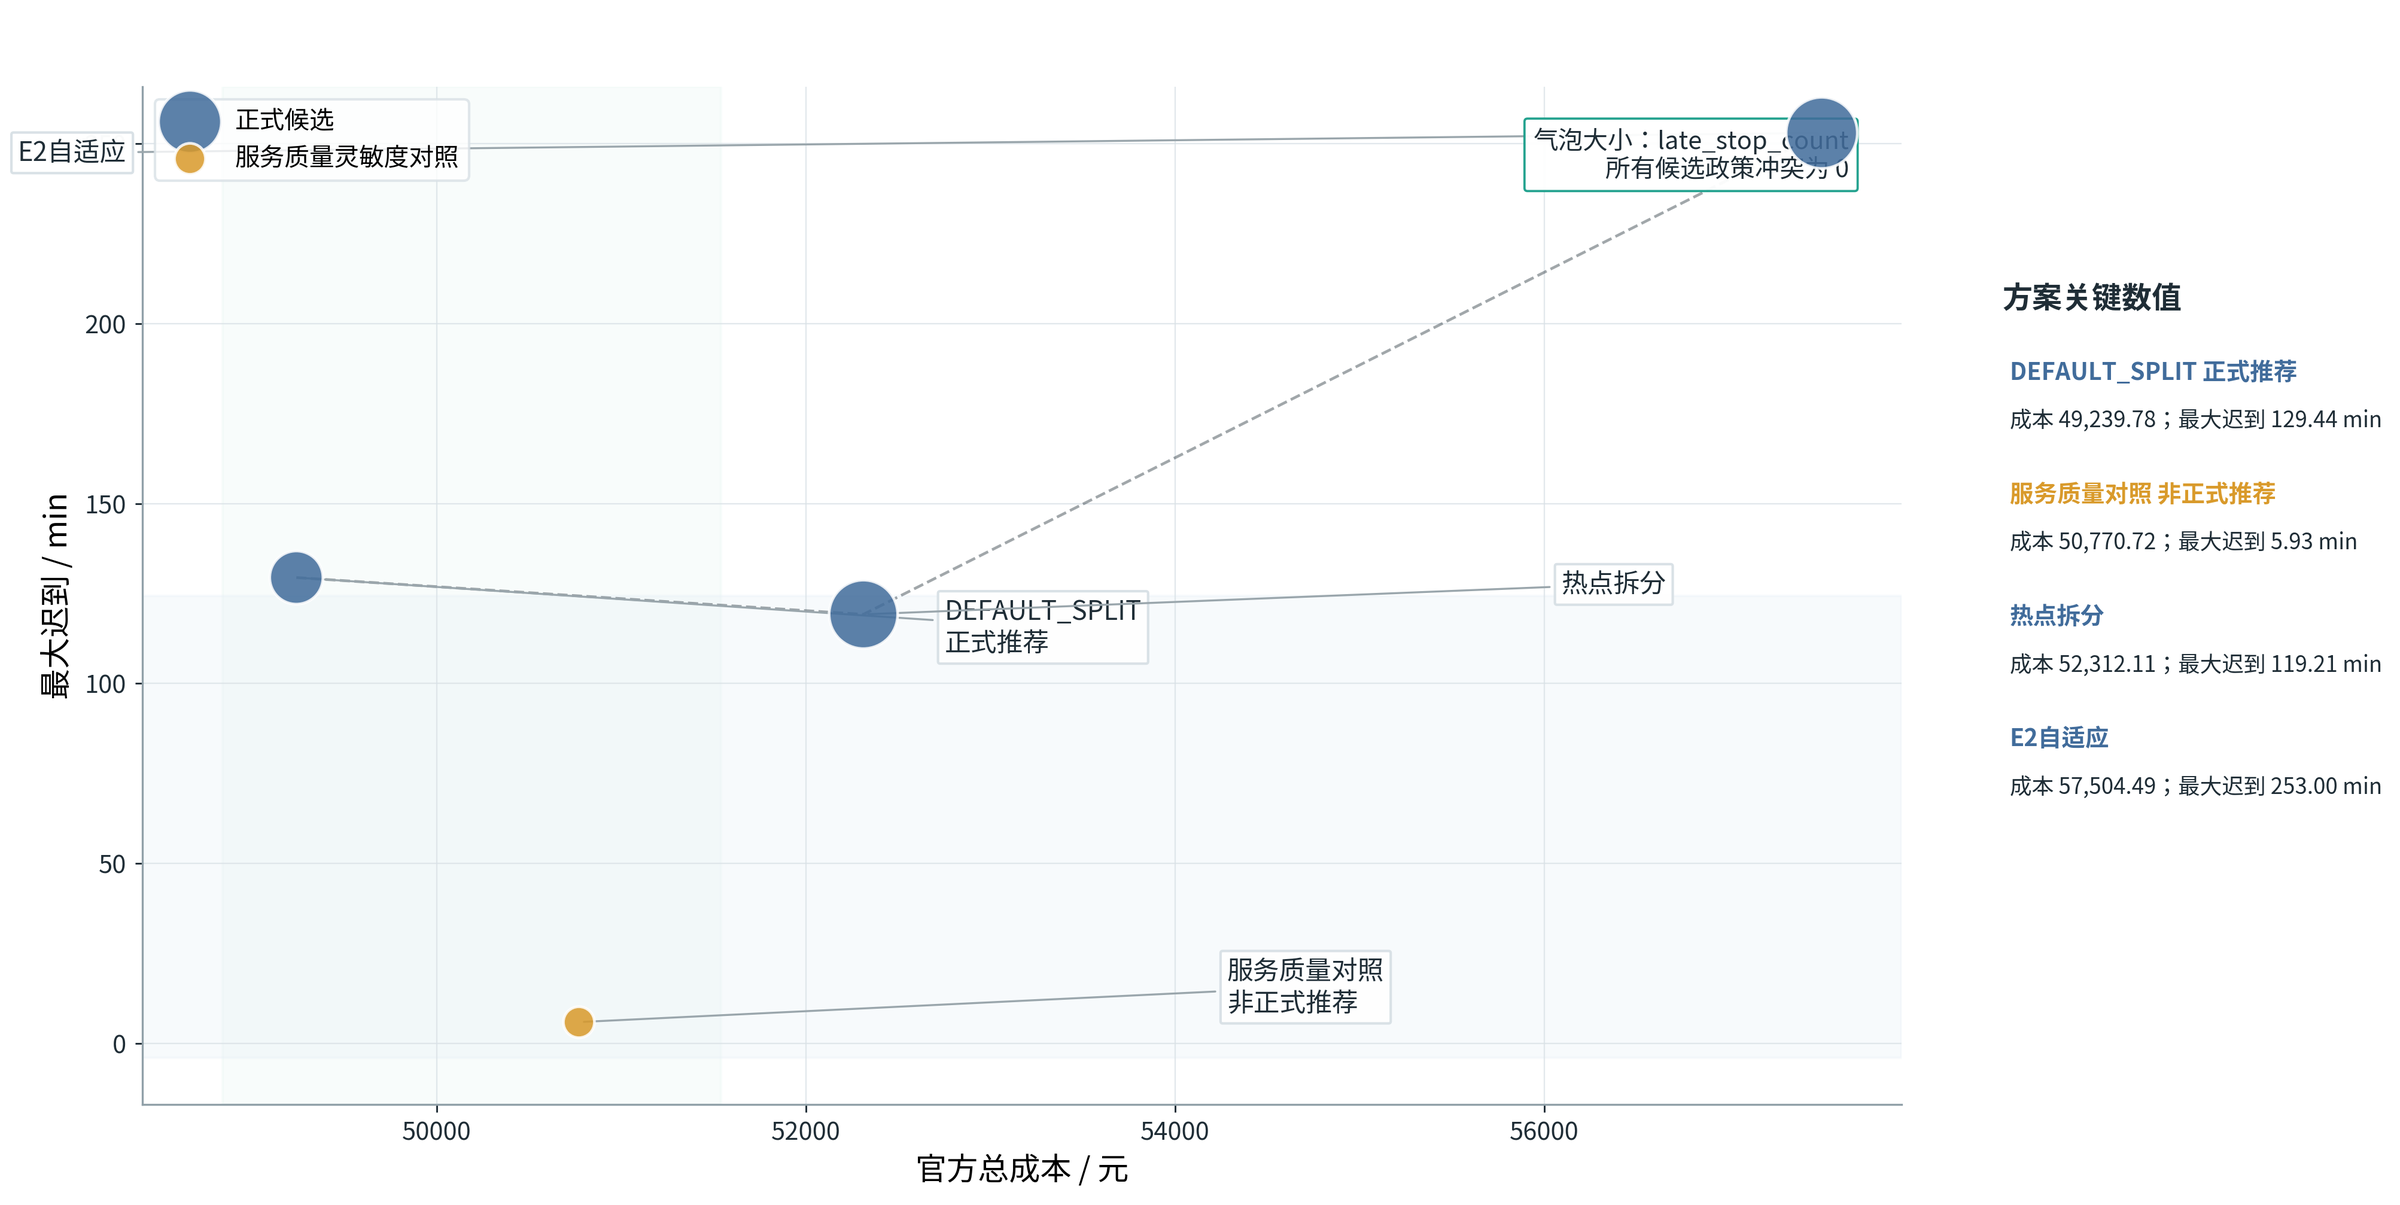
\includegraphics[width=0.95\textwidth]{fig07_problem2_cost_punctuality_pareto.png}
  \caption{第二问候选方案成本--准时性 Pareto 权衡。DEFAULT\_SPLIT 为正式成本推荐，服务质量对照方案仅用于灵敏度分析。}
  \label{fig:p2-pareto}
\end{figure}
\subsubsection{6.3.5 局限说明}

第二问不能判断燃油车真实道路是否穿越绿色区，只能检查服务事件合规；没有加入电动车续航、充电桩、充电排队和时变电价；绿色区细拆候选方案不是对所有可能拆分策略的穷举。正式方案的最大迟到体现成本优先解的服务边界，论文中通过服务质量对照方案给出可替代管理选择。

\subsection{6.4 第三问：事件驱动滚动时域动态响应模型}

\subsubsection{6.4.1 建模思路}

第三问以第二问正式方案为动态调度基准。事件发生时刻 \(t_e\) 将服务集合划分为

\[
S=S^{done}(t_e)\cup S^{lock}(t_e)\cup S^{free}(t_e).
\]

其中，\(S^{done}(t_e)\) 为已完成服务节点，不可撤销；\(S^{lock}(t_e)\) 为已出发趟次上的锁定节点，不能无条件跨车转移；\(S^{free}(t_e)\) 为未发车或未锁定的未来节点，可参与重排。新增订单构成 \(S^{new}(t_e)\)，取消订单构成 \(S^{cancel}(t_e)\)。变量说明如下：\(X^0\) 表示事件前基准方案，\(X\) 表示事件响应后方案；\(n_{\mathrm{change}}\) 表示服务位置或顺序变化节点数，\(n_{\mathrm{vehicle}}\) 表示换车节点数，\(n_{\mathrm{edge}}\) 表示被破坏的原连续服务边数量；这些扰动变量只用于解释动态响应稳定性，不进入官方成本。

动态调整后的官方成本仍为

\[
C(X)=C_{\mathrm{fixed}}(X)+C_{\mathrm{energy}}(X)+C_{\mathrm{carbon}}(X)+C_{\mathrm{tw}}(X).
\]

为了控制实时调度扰动，本文引入辅助稳定性指标

\[
D(X,X^0)=\alpha n_{\mathrm{change}}+\beta n_{\mathrm{vehicle}}+\gamma n_{\mathrm{edge}},
\]

其中 \(n_{\mathrm{change}}\) 为服务位置或顺序变化节点数，\(n_{\mathrm{vehicle}}\) 为换车节点数，\(n_{\mathrm{edge}}\) 为原连续服务边被破坏数量。该指标只用于候选筛选和解释，不进入题面官方成本。

\subsubsection{6.4.2 动态响应算法流程}

\begin{enumerate}[leftmargin=2em,itemsep=0.2em]
\item 读取第二问正式调度方案 \(X^0\)。
\item 在事件时刻 \(t_e\) 生成动态快照，识别已完成、锁定和可调整节点。
\item 根据事件类型更新残余需求池：取消订单删除未执行节点；新增订单创建代理服务节点；地址变更更新原服务节点映射；时间窗调整修改软时间窗参数。
\item 保持已完成和锁定部分不变。
\item 对残余池执行规则驱动快速修复，得到硬可行候选。
\item 在短预算内使用轻量 ALNS 对未冻结部分进行局部改进。
\item 验证覆盖、容量、物理车辆时间链和绿色限行政策。
\item 输出动态成本、成本变化、迟到水平和路线扰动指标。
\end{enumerate}

该流程的核心价值在于把“动态响应”从重新求解问题转化为带执行记忆的在线修复问题。已完成服务代表不可撤销事实，锁定趟次代表在途货物和司机任务边界，可调整池代表仍可由系统调度的未来计划。这样的分层能够解释为什么第三问不追求全天重排后的最低数值，而追求在硬可行、低扰动和可执行之间取得平衡。

第三问滚动响应的状态冻结逻辑可用图\ref{fig:dynamic-freezing-cube} 概括：事件时刻之前的事实不可逆，事件时刻之后的残余任务进入局部修复。

\begin{figure}[H]
  \centering
  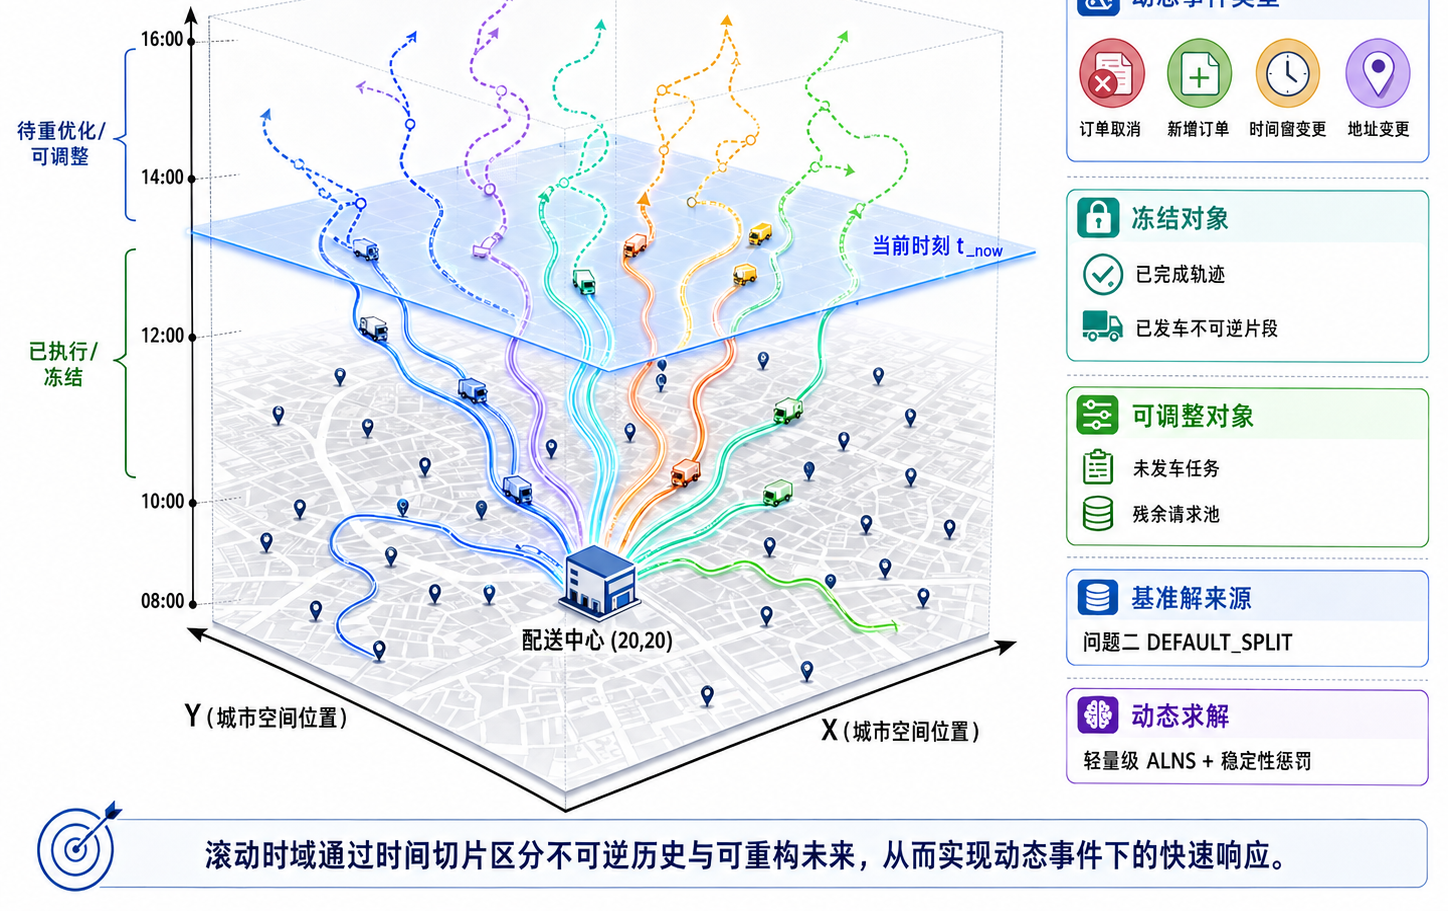
\includegraphics[width=0.92\textwidth]{fig08a_dynamic_freezing_cube.png}
  \caption{滚动时域下的状态冻结机制示意。该图为动态响应框架图，空间轨迹仅表示调度状态随时间的分层，不对应官方动态事件日志。}
  \label{fig:dynamic-freezing-cube}
\end{figure}

在具体路线层面，局部修复原则如图\ref{fig:dynamic-route-repair} 所示：冻结段保持不变，受影响的未来节点在原车辆和局部邻域内优先调整。

\begin{figure}[H]
  \centering
  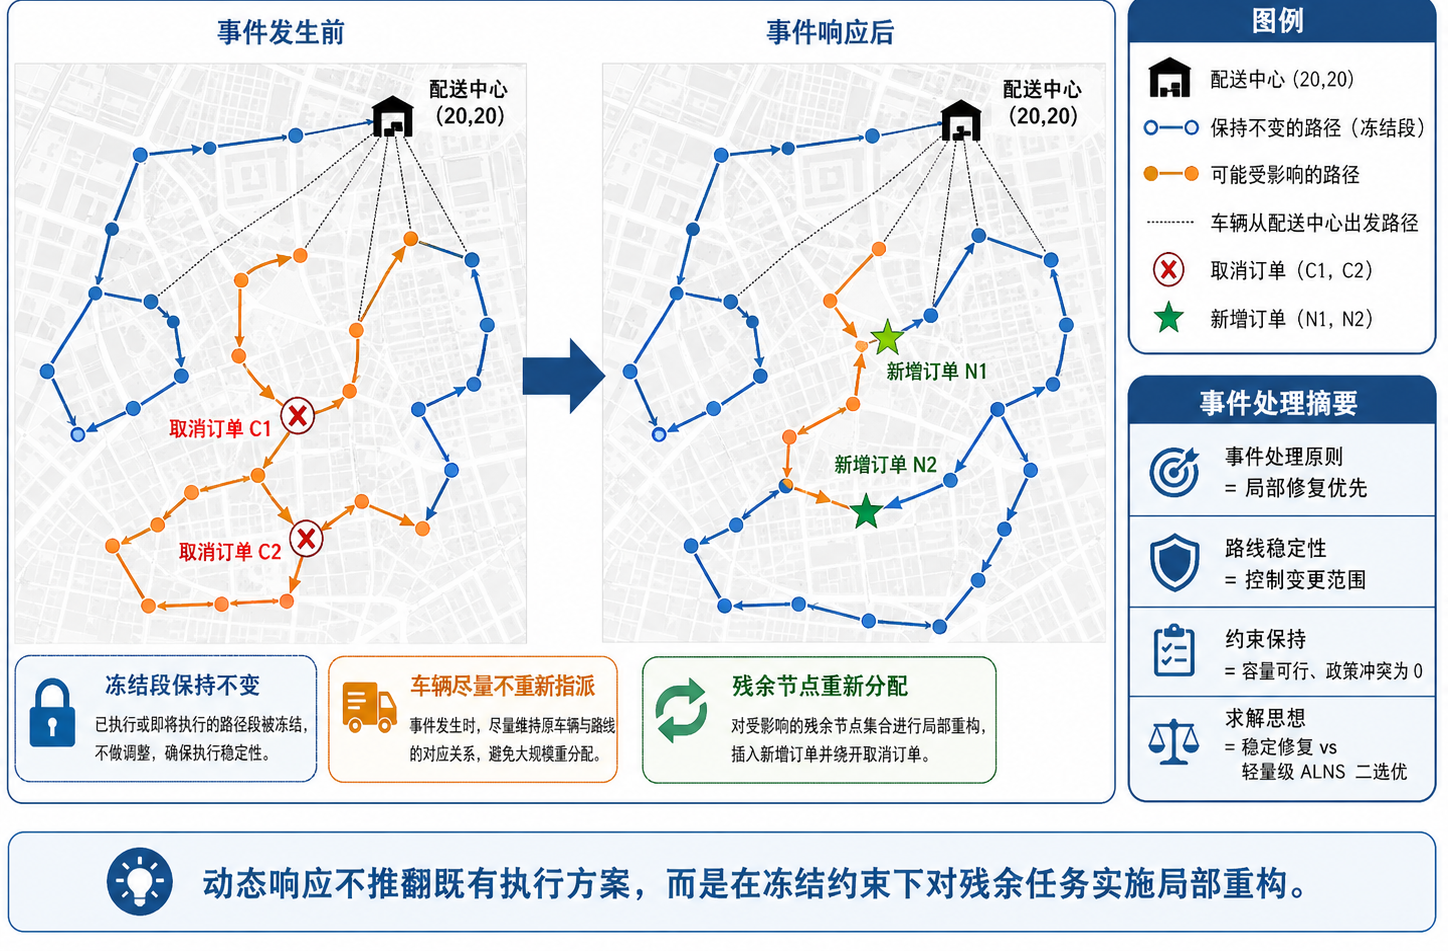
\includegraphics[width=0.92\textwidth]{fig08b_dynamic_route_reconstruction.png}
  \caption{动态事件前后的局部路线重构示意。该图仅说明新增与取消事件下的局部修复逻辑，不代表第三问四个情景的官方事件记录或真实道路轨迹。}
  \label{fig:dynamic-route-repair}
\end{figure}

动态事件发生后的事实冻结与滚动修复时间轴见图\ref{fig:p3-frozen-gantt}。

\begin{figure}[H]
  \centering
  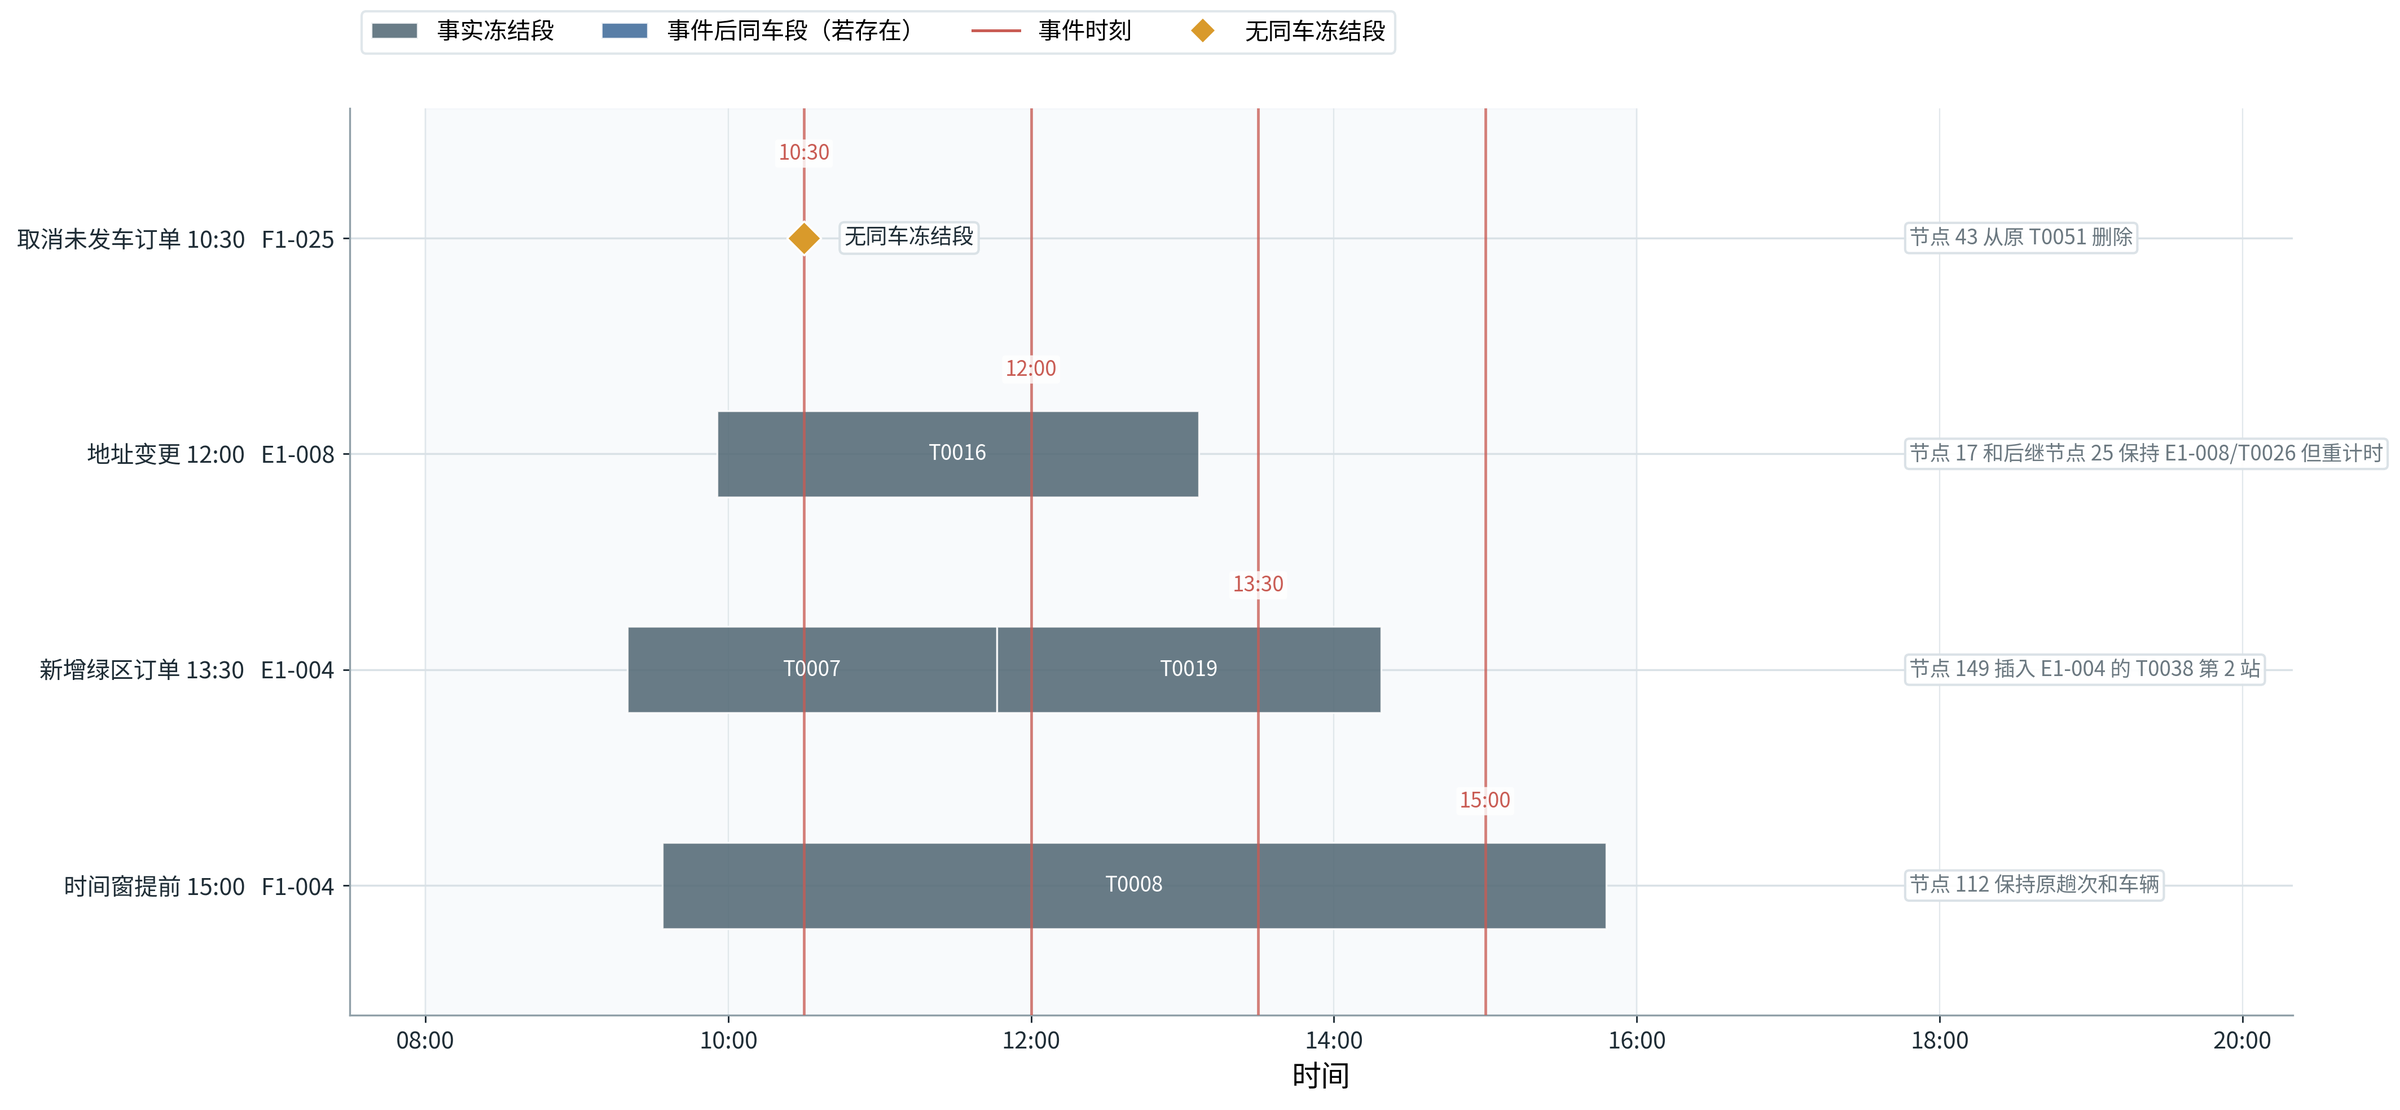
\includegraphics[width=0.96\textwidth]{fig08_problem3_frozen_gantt.png}
  \caption{基于事实冻结的滚动时域车辆时间轴。事件线左侧表示已执行或锁定事实，右侧未来服务池参与局部修复。}
  \label{fig:p3-frozen-gantt}
\end{figure}
\subsubsection{6.4.3 代表性情景设计}

由于题面没有具体动态事件数据，本文构造四个代表性情景，覆盖题面四类突发事件。情景均记录在 \texttt{outputs/problem3/scenario\_assumptions.csv} 中。

\begin{table}[H]
\centering
\small
\caption{第三问代表性动态情景设计}
\label{tab:p3-scenarios}
\begin{tabularx}{\textwidth}{>{\raggedright\arraybackslash}X>{\raggedright\arraybackslash}X>{\raggedright\arraybackslash}X>{\raggedright\arraybackslash}X>{\raggedright\arraybackslash}X}
\toprule
情景 & 事件时刻 & 事件类型 & 假设内容 & 设计目的 \\
\midrule
cancel\_future\_order\_1030 & 630 (10:30) & 订单取消 & 取消一个尚未发车趟次中的服务节点 43 & 检验未执行订单删除与成本下降 \\
new\_green\_order\_1330 & 810 (13:30) & 新增订单 & 新增绿色区代理节点 149，代理客户 9，需求 300 kg / 1.0 m\(^3\)，时间窗 14:00-17:00 & 检验绿色新增订单的政策合规插入 \\
time\_window\_pull\_forward\_1500 & 900 (15:00) & 时间窗调整 & 将尚未服务节点 112 的时间窗调整为 18:52-19:46 & 检验时间窗收紧对罚金影响 \\
address\_change\_proxy\_1200 & 720 (12:00) & 地址变更 & 将尚未服务节点 17 的配送地址改为既有客户 12 的位置 & 检验无新距离矩阵时的代理改址 \\
\bottomrule
\end{tabularx}
\end{table}

\subsubsection{6.4.4 动态结果}

四个代表性情景的正式结果见表\ref{tab:p3-result}。

\begin{table}[H]
\centering
\small
\caption{第三问动态响应结果}
\label{tab:p3-result}
\begin{tabularx}{\textwidth}{>{\raggedright\arraybackslash}X>{\raggedright\arraybackslash}X>{\raggedright\arraybackslash}X>{\raggedright\arraybackslash}X>{\raggedright\arraybackslash}X>{\raggedright\arraybackslash}X>{\raggedright\arraybackslash}X>{\raggedright\arraybackslash}X>{\raggedright\arraybackslash}X>{\raggedright\arraybackslash}X>{\raggedright\arraybackslash}X}
\toprule
情景 & 动态成本/元 & 相对第二问/元 & 固定成本 & 能源成本 & 碳排成本 & 时间窗罚金 & 政策冲突 & 迟到点 / 最大迟到 & 调整节点 & 换车节点 \\
\midrule
订单取消 & 48711.28 & -528.51 & 18000.00 & 24117.82 & 5207.29 & 1386.17 & 0 & 12 / 129.44 & 1 & 0 \\
新增绿区订单 & 49237.36 & -2.42 & 18000.00 & 24549.88 & 5301.32 & 1386.17 & 0 & 12 / 129.44 & 2 & 0 \\
时间窗提前 & 49263.35 & +23.57 & 18000.00 & 24551.90 & 5301.72 & 1409.74 & 0 & 13 / 129.44 & 1 & 0 \\
地址变更 & 49207.47 & -32.31 & 18000.00 & 24533.45 & 5298.06 & 1375.97 & 0 & 12 / 129.44 & 2 & 0 \\
\bottomrule
\end{tabularx}
\end{table}

四个代表性动态情景的成本响应与扰动规模见图\ref{fig:p3-response-matrix}。

\begin{figure}[H]
  \centering
  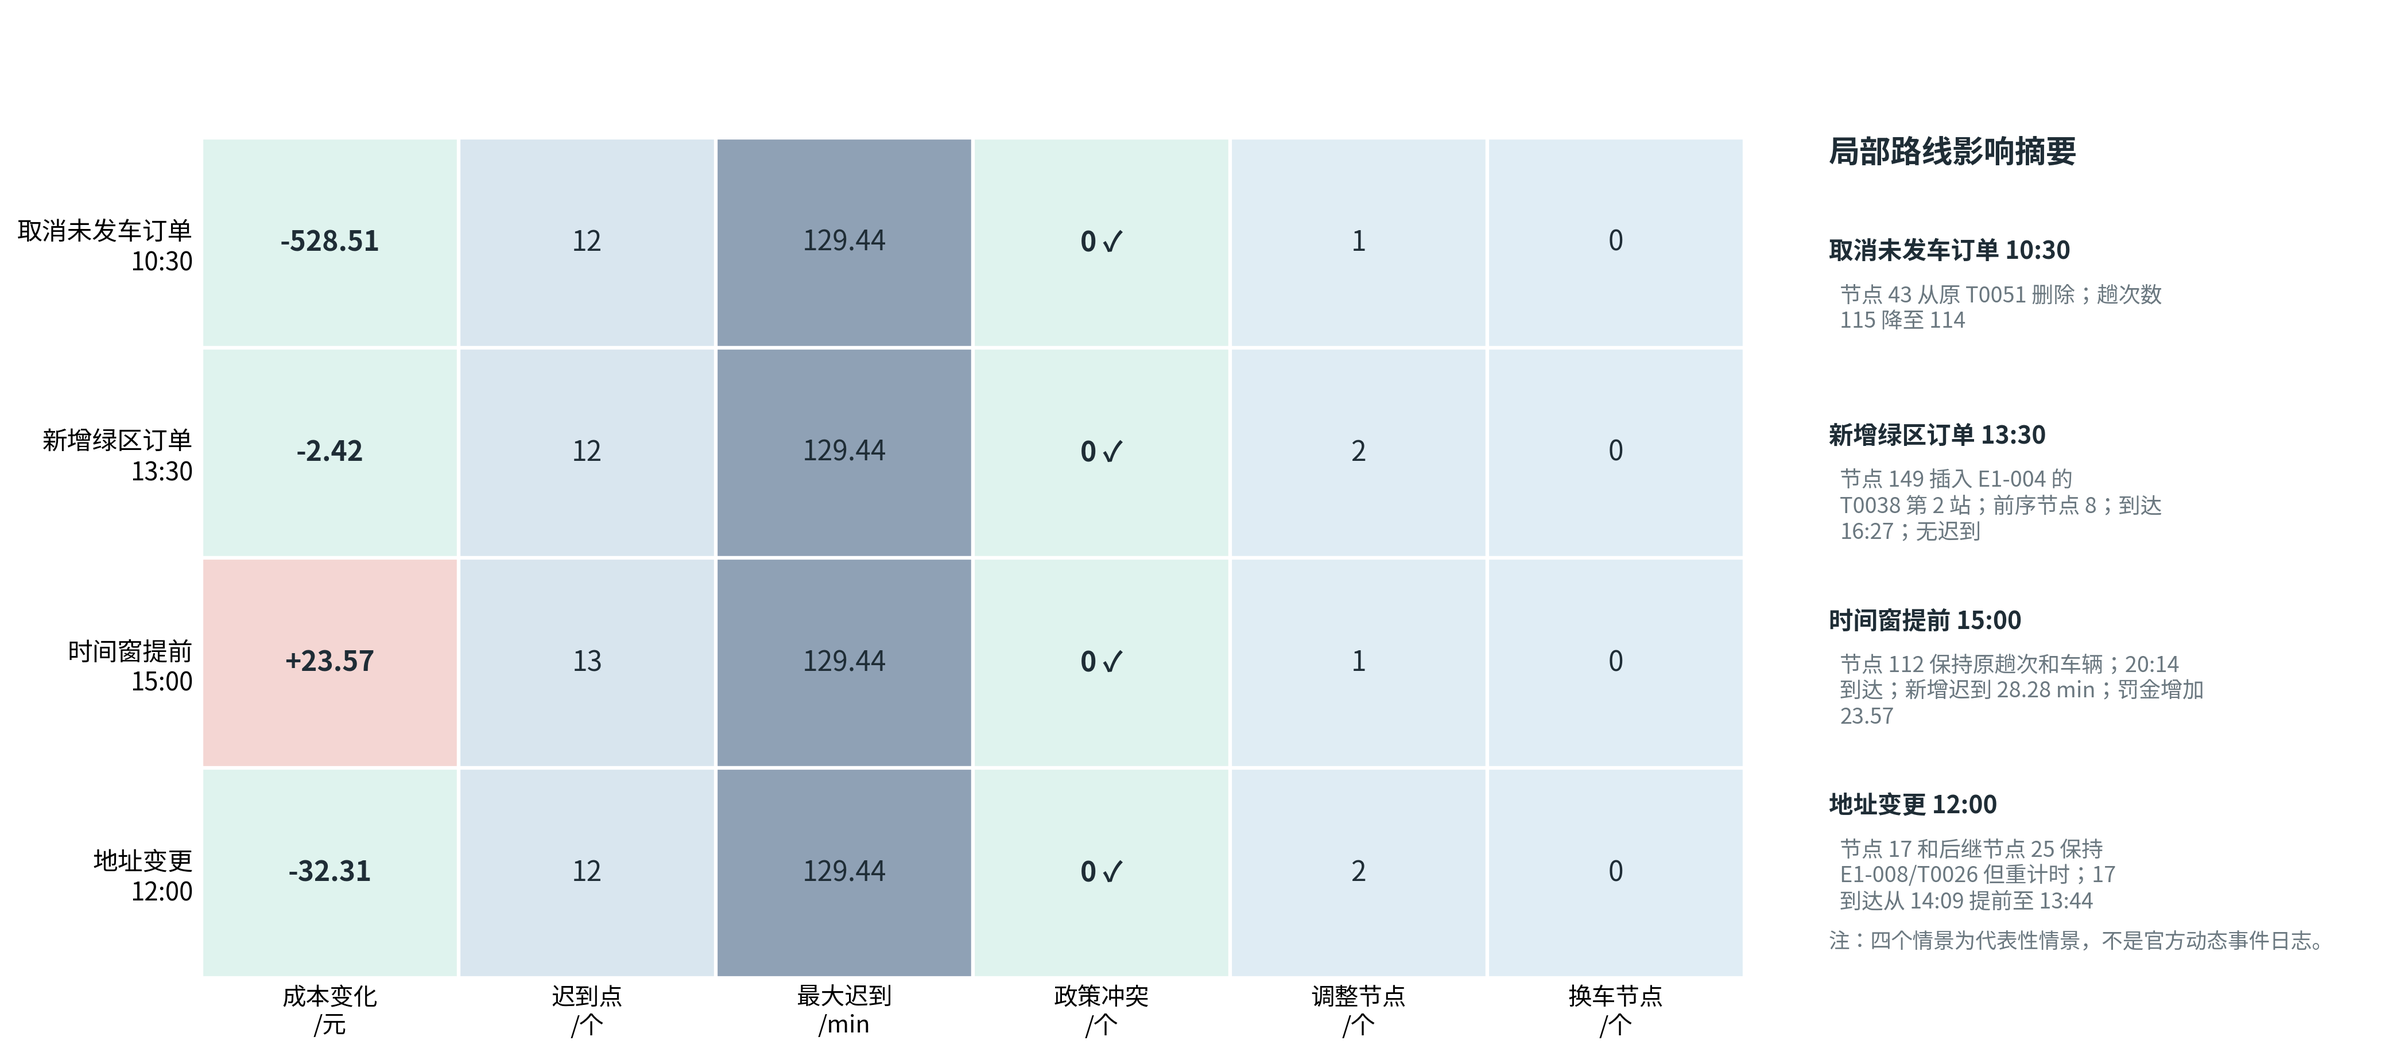
\includegraphics[width=0.96\textwidth]{fig09_problem3_event_response_matrix.png}
  \caption{第三问动态事件响应成本--扰动矩阵。四个情景为代表性动态扰动，均保持硬可行且政策冲突为 0。}
  \label{fig:p3-response-matrix}
\end{figure}
\subsubsection{6.4.5 结果解释}

订单取消情景总成本下降 \texttt{528.51} 元，主要来自未执行服务节点删除后行驶距离、能源消耗和碳排放减少。时间窗提前情景总成本增加 \texttt{23.57} 元，且迟到点从 12 个增至 13 个，说明时间窗扰动主要通过软时间窗罚金影响成本。

新增绿区订单情景总成本略降 \texttt{2.42} 元，不应解释为新增订单必然降低成本。该结果来自代理节点插入后对原路线等待结构的重分配：新增服务占用了局部空余时间和车辆容量，同时改变了后续等待与出发时刻，使能源、碳排与时间窗罚金发生小幅抵消；该结论只对当前代理客户 9 和当前路线结构成立，不具备普遍方向性。地址变更情景成本下降 \texttt{32.31} 元，也只表示代理客户 12 在当前距离结构下更接近原路线。四个情景的共同结论是：滚动响应策略能在不产生政策冲突、不破坏容量和物理车辆时间链的前提下，对突发事件给出可执行调整。

从扰动角度看，四个情景调整节点数均不超过 2，换车节点数均为 0，说明事件响应主要通过残余节点的局部插入、删除或时间窗修正完成，没有大规模改派车辆。该性质对实际运营较有价值：调度系统既能响应突发变化，又能保持司机任务和客户沟通的稳定性。由于这些扰动指标不属于题面官方成本，本文仅将其作为动态方案解释证据。

\subsubsection{6.4.6 局限说明}

第三问没有官方动态事件日志，因此本文不能进行真实事件回放；新增订单和地址变更使用既有客户点代理，没有生成新距离矩阵；当前策略偏向稳定修复，未声明动态全局最优；模型未处理在途车辆精确位置插值、中途换装或路边转运。


\section{七、模型检验与敏感性分析}

\subsection{7.1 硬可行性检验}

本文从覆盖、容量、物理车辆时间链和政策冲突四个方面检验正式结果。第一问和第二问全部虚拟服务节点均被服务一次，无缺失和重复；第三问四个代表性情景中，除取消节点外，所有应服务节点均被覆盖。所有路线均满足重量和体积容量，物理车辆连续趟次不重叠。第二问和第三问政策冲突均为 0。

\begin{table}[H]
\centering
\small
\caption{硬可行性检验汇总}
\label{tab:validation}
\begin{tabularx}{\textwidth}{>{\raggedright\arraybackslash}X>{\raggedright\arraybackslash}X>{\raggedright\arraybackslash}X>{\raggedright\arraybackslash}X>{\raggedright\arraybackslash}X>{\raggedright\arraybackslash}X}
\toprule
检验对象 & 覆盖可行 & 容量可行 & 物理车辆链可行 & 政策冲突 & 迟到点 / 最大迟到 \\
\midrule
第一问正式解 & 是 & 是 & 是 & 不适用 & 4 / 31.60 min \\
第二问正式解 & 是 & 是 & 是 & 0 & 12 / 129.44 min \\
第三问订单取消 & 是 & 是 & 是 & 0 & 12 / 129.44 min \\
第三问新增绿区订单 & 是 & 是 & 是 & 0 & 12 / 129.44 min \\
第三问时间窗提前 & 是 & 是 & 是 & 0 & 13 / 129.44 min \\
第三问地址变更 & 是 & 是 & 是 & 0 & 12 / 129.44 min \\
\bottomrule
\end{tabularx}
\end{table}

全题关键约束检验结果见图\ref{fig:validation-dashboard}。

\begin{figure}[H]
  \centering
  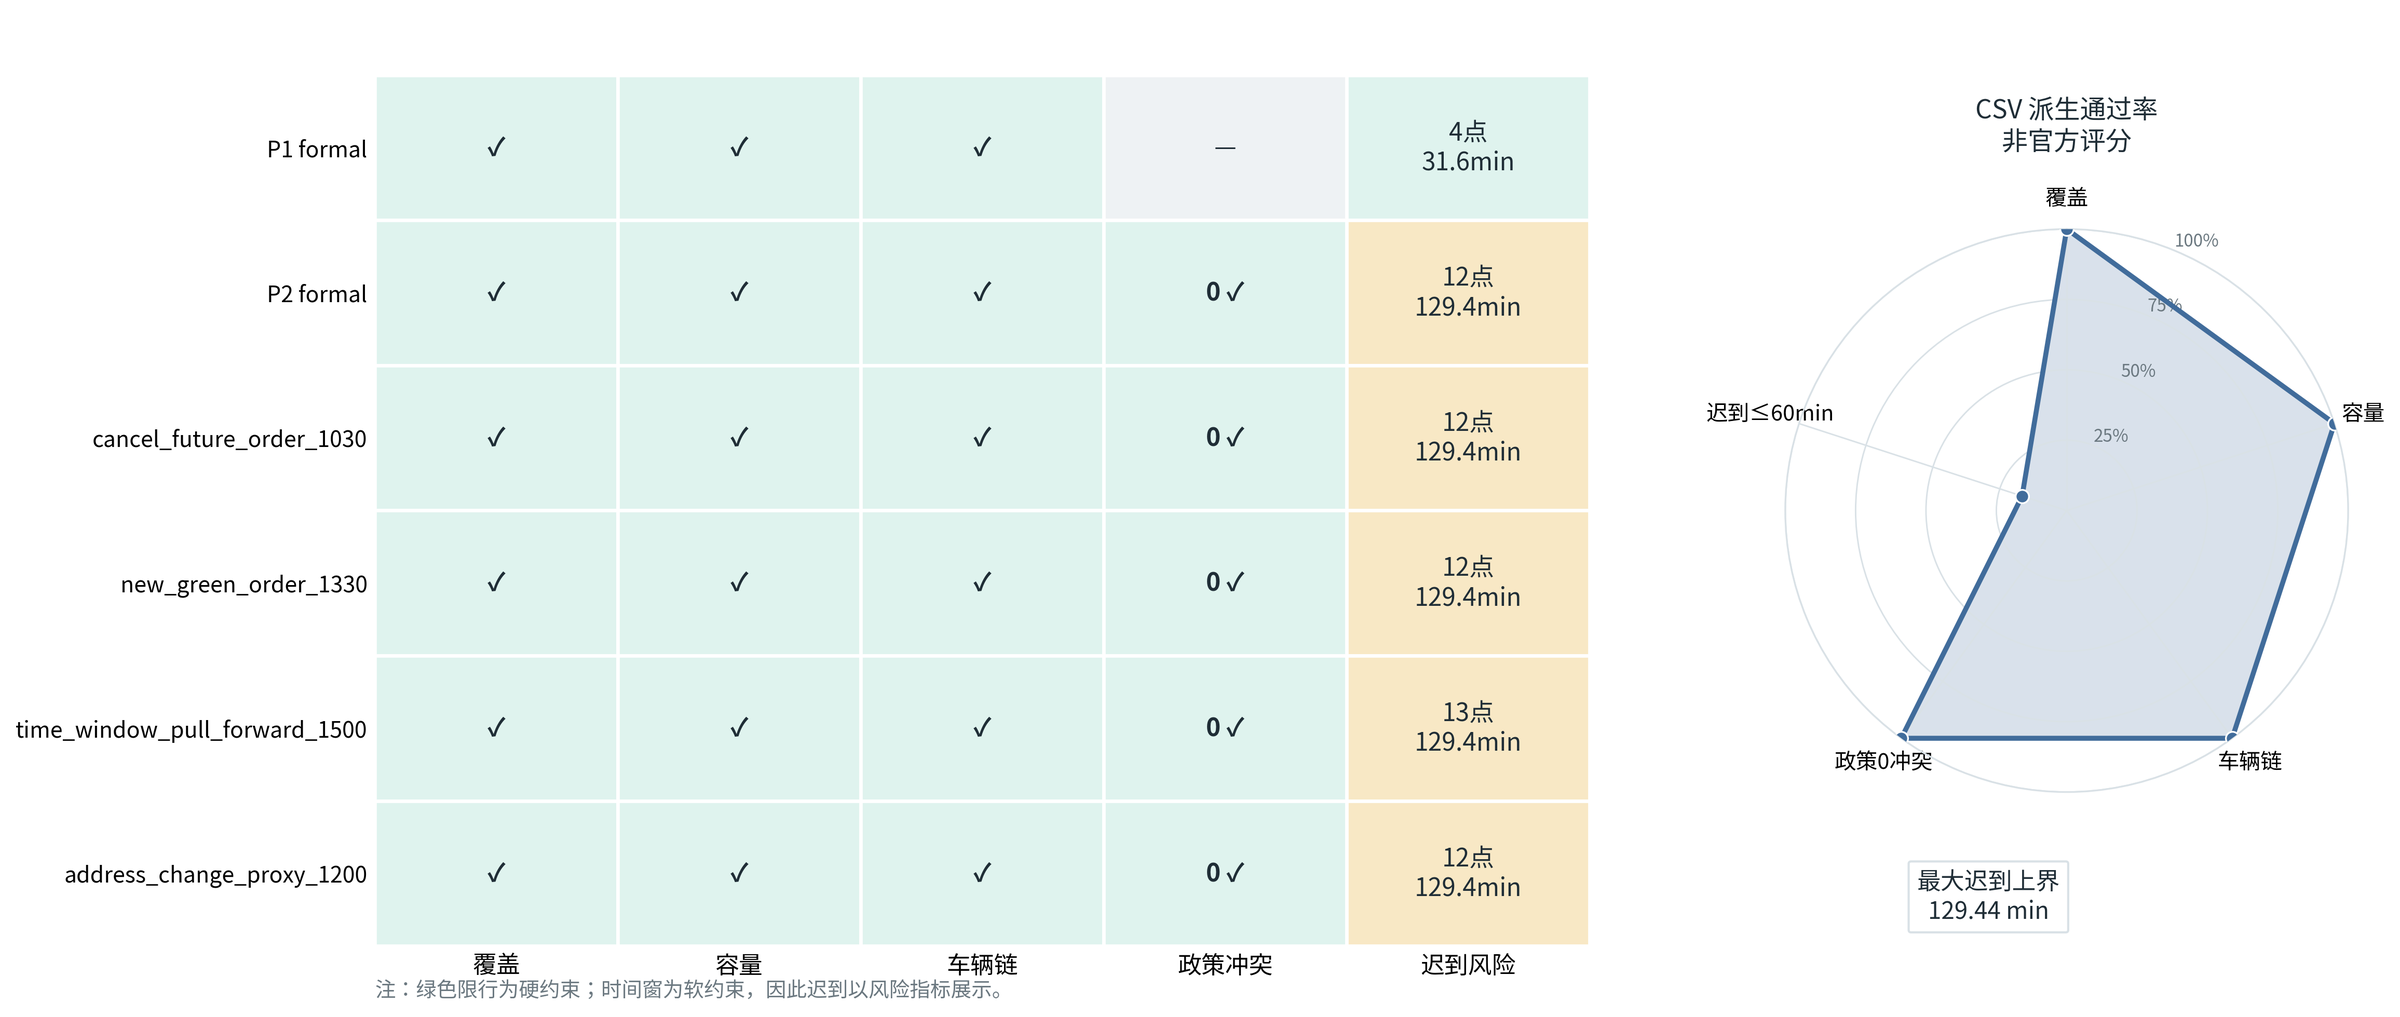
\includegraphics[width=0.96\textwidth]{fig10_feasibility_validation_dashboard.png}
  \caption{全题模型可信性检验矩阵。硬约束通过项与软时间窗迟到风险分列展示，避免将迟到误判为不可行。}
  \label{fig:validation-dashboard}
\end{figure}
\subsection{7.2 成本重构检验}

第一问总成本由 \texttt{17200.00+25091.79+5419.37+933.53=48644.68} 元构成；第二问总成本由 \texttt{18000.00+24551.90+5301.72+1386.17=49239.78} 元构成。第三问各情景也均由固定成本、能源成本、碳排成本和软时间窗罚金四项重构。政策冲突、EV reservation、稳定性指标和路线扰动指标均未进入官方成本。

\subsection{7.3 第一问稳定性与迟到诊断}

第一问正式运行 40 次 ALNS 迭代得到 \texttt{48644.68} 元。同 seed 的 100 迭代审计未找到更低官方总成本，可说明当前解在该 seed 和邻域设置下没有明显早停风险，但不能证明全局最优。

第一问 4 个残余迟到点被分为三类：直达也迟到、多趟物理车辆级联、路线顺序局部问题。该诊断说明时间窗约束并未遗漏，迟到是软时间窗成本权衡后的结果。若后续引入“准时率优先”的管理目标，应另建多目标或约束版本，不应改写本题官方成本模型。

\subsection{7.4 第二问政策结构与服务质量权衡}

第二问候选比较显示，盲目将绿色区客户细拆并不必然降低总成本。\texttt{GREEN\_E2\_ADAPTIVE} 虽增加了 E2 参与可能，但服务节点增多后固定成本和排班复杂度上升，总成本达到 \texttt{57504.49} 元，能源成本和碳排成本分别为 \texttt{25199.05} 元和 \texttt{5444.15} 元，均高于默认拆分。\texttt{GREEN\_HOTSPOT\_PARTIAL} 是更温和的局部细拆，但其能源成本和碳排成本分别升至 \texttt{26832.05} 元和 \texttt{5797.39} 元，总成本仍为 \texttt{52312.11} 元，高于默认拆分。

服务质量对照方案证明迟到风险可以显著降低：最大迟到由 \texttt{129.44 min} 降为 \texttt{5.93 min}，迟到点由 12 个降为 2 个，但成本提高至 \texttt{50770.72} 元。这一结果应写作灵敏度分析，说明成本目标和准时性目标存在可量化冲突。

\subsection{7.5 第三问动态事件响应检验}

第三问四类事件均保持硬可行和政策冲突为 0。取消订单成本下降、时间窗提前成本上升，符合事件对需求量和时间压力的直观影响。新增订单和地址变更的成本方向依赖局部路线结构，不能概括为固定规律。四个情景的换车节点数均为 0，调整节点数不超过 2，说明当前滚动响应策略偏向低扰动修复，适合实时运营解释。

\subsection{7.6 误差来源分析}

\begin{table}[H]
\centering
\small
\caption{误差来源与控制方式}
\label{tab:error-sources}
\begin{tabularx}{\textwidth}{>{\raggedright\arraybackslash}X>{\raggedright\arraybackslash}X>{\raggedright\arraybackslash}X}
\toprule
误差来源 & 影响 & 本文处理 \\
\midrule
17:00 后速度分布缺失 & 影响晚间 ETA、能耗和迟到罚金 & 延用一般时段速度，并在假设中披露 \\
无道路几何 & 不能判断真实道路穿越绿色区 & 只检查绿色区客户服务事件合规 \\
启发式无全局下界 & 不能证明全局最优 & 用收敛审计、候选对比和硬可行性验证支撑 \\
客户拆分假设 & 改变服务颗粒 & 保留 \texttt{service\_node\_id -> customer\_id} 映射 \\
第三问无官方事件数据 & 不能进行真实事件复盘 & 明确写作代表性情景假设 \\
\bottomrule
\end{tabularx}
\end{table}

若后续时间允许，可在固定路线结构下进行速度随机回放，比较随机仿真均值与当前期望模型成本；该实验当前未作为正式结果，因此正文不报告具体随机鲁棒性数值。


\section{八、模型评价与改进方向}

模型评价从题意贴合度、物理一致性、求解可复核性和运营可解释性四个方面展开。本文不以“复杂模型堆叠”作为优势，而以每个模型部件均能对应题目数据或管理约束作为评价标准。

\subsection{8.1 模型优点}

第一，目标与约束边界清晰。本文始终将官方成本限定为固定成本、能源成本、碳排成本和软时间窗罚金，绿色限行作为硬约束，服务质量和路线扰动作为诊断指标。这一边界使三问结果能够横向比较，也避免把政策冲突或搜索辅助项误写成成本。

第二，物理解释较强。分段积分处理时变行驶时间，Jensen 修正处理速度随机性下的二次能耗，载重率修正连接路线顺序和能耗碳排。由此，模型能够解释“同样距离在不同时段、不同载重下成本不同”这一题面核心机制。

第三，数据结构与附件边界一致。虚拟服务节点解决超容量需求，原始 customer\_id 保证距离矩阵索引正确；绿色区按 \((0,0)\) 坐标判定，配送中心 \((20,20)\) 不与城市中心混淆。该处理减少了建模层面最容易出现的索引错配和空间概念错用风险。

第四，物理车辆多趟复用提高了可行性。模型区分 depot-to-depot 趟次和启用物理车辆，既符合大量需求数据，也符合固定成本按车辆计的题意，使“路线数多”与“启用车辆数少”能够同时被解释。

第五，第三问动态响应可审计。事件发生后冻结已执行事实，只调整未执行部分，避免货物瞬移和全天推倒重排，并能通过调整节点数、换车节点数等指标解释调度稳定性。

第六，结果体系完整。正式结果、服务质量对照、模型检验、图表数据包和支撑材料边界分明，便于复核和论文排版。

\subsection{8.2 模型适用边界}

第一，ALNS 启发式不能给出全局最优证明。

第二，模型没有道路几何，无法做道路级绿色区穿越检测。

第三，17:00 后速度分布依赖延拓假设。

第四，新能源车辆运营被简化，没有显式建模 SOC、续航、充电桩、充电排队和时变电价。

第五，第三问没有官方动态事件数据，只能用代表性情景展示方法。

第六，第二问成本优先方案与准时优先方案存在明确取舍。本文已通过服务质量对照方案量化该边界，但正式推荐仍按题面官方成本最小准则确定。

\subsection{8.3 改进方向}

后续可从六个方向扩展：一是建立小规模精确模型或列生成下界，用于校准启发式解质量；二是在获得 GIS 路网后升级为道路级绿色区限行检测；三是加入电动车 SOC、充电调度和时变电价；四是开展固定路线下的速度蒙特卡洛回放，检验期望能耗模型鲁棒性；五是若获得真实动态订单流，构建在线仿真评估体系；六是在官方成本模型之外建立多目标管理版本，同时控制成本、碳排和准时率，并与本文主模型分开报告。


\begin{thebibliography}{99}
\bibitem{ropke2006alns} Ropke S, Pisinger D. An adaptive large neighborhood search heuristic for the pickup and delivery problem with time windows[J]. Transportation Science, 2006, 40(4):455--472.
\bibitem{pisinger2007general} Pisinger D, Ropke S. A general heuristic for vehicle routing problems[J]. Computers \& Operations Research, 2007, 34(8):2403--2435.
\bibitem{ichoua2003time} Ichoua S, Gendreau M, Potvin J Y. Vehicle dispatching with time-dependent travel times[J]. European Journal of Operational Research, 2003, 144(2):379--396.
\bibitem{bektas2011pollution} Bektaş T, Laporte G. The pollution-routing problem[J]. Transportation Research Part B: Methodological, 2011, 45(8):1232--1250.
\bibitem{demir2012alns} Demir E, Bektaş T, Laporte G. An adaptive large neighborhood search heuristic for the pollution-routing problem[J]. European Journal of Operational Research, 2012, 223(2):346--359.
\bibitem{erdogan2012green} Erdoğan S, Miller-Hooks E. A green vehicle routing problem[J]. Transportation Research Part E: Logistics and Transportation Review, 2012, 48(1):100--114.
\bibitem{schneider2014evrptw} Schneider M, Stenger A, Goeke D. The electric vehicle-routing problem with time windows and recharging stations[J]. Transportation Science, 2014, 48(4):500--520.
\bibitem{goeke2015mixed} Goeke D, Schneider M. Routing a mixed fleet of electric and conventional vehicles[J]. European Journal of Operational Research, 2015, 245(1):81--99.
\bibitem{bent2004scenario} Bent R, Van Hentenryck P. Scenario-based planning for partially dynamic vehicle routing with stochastic customers[J]. Operations Research, 2004, 52(6):977--987.
\bibitem{pillac2013review} Pillac V, Gendreau M, Guéret C, Medaglia A L. A review of dynamic vehicle routing problems[J]. European Journal of Operational Research, 2013, 225(1):1--11.
\end{thebibliography}

\clearpage
\appendix
\section{附录说明}

\subsection{附录 A：支撑材料文件列表}

支撑材料与论文 PDF 分开提交，承诺书不放入论文和支撑材料。支撑材料中不包含身份相关信息，主要文件见表\ref{tab:support-files}。

\begin{table}[H]
\centering
\small
\caption{支撑材料文件列表}
\label{tab:support-files}
\begin{tabularx}{\textwidth}{>{\raggedright\arraybackslash}X>{\raggedright\arraybackslash}X>{\raggedright\arraybackslash}X}
\toprule
类型 & 路径 & 说明 \\
\midrule
LaTeX 源文件 & \texttt{paper/hzcup\_a\_final\_paper.tex} & 论文可编辑源文件 \\
论文图片 & \texttt{paper/figures/} & 正文图像文件 \\
核心程序 & \texttt{green\_logistics/} & 数据处理、成本评价、调度搜索与动态响应模块 \\
三问入口 & \texttt{problems/problem1.py}，\texttt{problems/problem2.py}，\texttt{problems/problem3.py} & 第一至第三问复现入口 \\
实验入口 & \texttt{problems/experiments/} & 第二问服务质量对照与参数对比程序 \\
正式结果 & \texttt{outputs/problem1/}，\texttt{outputs/problem2/}，\texttt{outputs/problem3/} & 三问正式输出结果 \\
模型检验 & \texttt{outputs/model\_validation/} & 可行性、成本重构和敏感性检验结果 \\
图表数据 & \texttt{outputs/figure\_data/} & 正文图像所用表格数据与导出图像 \\
测试程序 & \texttt{tests/} & 单元测试与集成测试 \\
\bottomrule
\end{tabularx}
\end{table}

\subsection{附录 B：可复现命令}

\begin{lstlisting}[basicstyle=\ttfamily\footnotesize,breaklines=true]
python problems/problem1.py --iterations 40 --remove-count 8 --seed 20260424 --output-dir outputs/problem1
python problems/problem2.py --iterations 40 --remove-count 16 --seed 20260427 --use-ev-reservation --ev-reservation-penalty 250 --output-dir outputs/problem2
python problems/experiments/problem2_parameter_sweep.py --iterations 40 --remove-counts 16 --seeds 20260427 --variants default_split --use-policy-operators --use-ev-reservation --ev-reservation-penalty 500 --output-dir outputs/problem2_experiments/formal_screen_policy_ev_p500
python problems/problem3.py --iterations 8 --remove-count 4 --seed 20260426 --output-dir outputs/problem3 --no-plots
pytest -q
\end{lstlisting}

\subsection{附录 C：关键实现代码摘录}

完整可运行源程序随支撑材料提交，本文仅摘录与模型机制直接相关的关键实现。

\begin{lstlisting}[language=Python,basicstyle=\ttfamily\footnotesize,breaklines=true]
def green_zone(customer):
    x, y = customer.x, customer.y
    return x * x + y * y <= 100

def policy_feasible(node, vehicle_type, arrival):
    if vehicle_type in FUEL_TYPES and node.green and 480 <= arrival < 960:
        return False
    return True

def split_customer(customer, max_weight=3000.0, max_volume=15.0):
    n = ceil(max(customer.weight / max_weight, customer.volume / max_volume))
    return [
        ServiceNode(customer.id, customer.weight / n, customer.volume / n,
                    customer.tw_start, customer.tw_end, customer.x, customer.y)
        for _ in range(n)
    ]
\end{lstlisting}

\begin{lstlisting}[language=Python,basicstyle=\ttfamily\footnotesize,breaklines=true]
def expected_energy(kind, mu, sigma):
    ev2 = mu * mu + sigma * sigma
    if kind == "fuel":
        return 0.0025 * ev2 - 0.2554 * mu + 31.75
    return 0.0014 * ev2 - 0.12 * mu + 36.19

def arc_energy(kind, distance, segments, load_ratio):
    factor = 1.0 + (0.40 if kind == "fuel" else 0.35) * load_ratio
    energy = 0.0
    for seg_distance, mu, sigma in segments:
        energy += seg_distance / 100.0 * expected_energy(kind, mu, sigma)
    return factor * energy

def soft_time_window_cost(arrival, tw_start, tw_end):
    wait = max(tw_start - arrival, 0.0)
    late = max(arrival - tw_end, 0.0)
    return 20.0 / 60.0 * wait + 50.0 / 60.0 * late
\end{lstlisting}

\begin{lstlisting}[language=Python,basicstyle=\ttfamily\footnotesize,breaklines=true]
def evaluate_route(route, vehicle):
    time = route.departure
    load = sum(node.weight for node in route.nodes)
    cost = 0.0
    carbon = 0.0
    prev = DEPOT
    for node in route.nodes + [DEPOT]:
        segments = time_dependent_segments(prev.customer_id, node.customer_id, time)
        load_ratio = load / vehicle.capacity_weight
        e = arc_energy(vehicle.energy_kind, distance(prev, node), segments, load_ratio)
        time += travel_time(segments)
        cost += energy_price(vehicle.energy_kind) * e
        carbon += emission_factor(vehicle.energy_kind) * e
        if node is not DEPOT:
            cost += soft_time_window_cost(time, node.tw_start, node.tw_end)
            time = max(time, node.tw_start) + 20.0
            load -= node.weight
        prev = node
    return cost, carbon, time
\end{lstlisting}

\begin{lstlisting}[language=Python,basicstyle=\ttfamily\footnotesize,breaklines=true]
def dynamic_repair(base_solution, event_time, event):
    done, locked, free = freeze_state(base_solution, event_time)
    pool = update_pool(free, event)
    candidate = greedy_repair(locked, pool)
    best = candidate
    for _ in range(LOCAL_ITERATIONS):
        removed = destroy(best)
        trial = repair(removed, locked)
        if hard_feasible(trial) and objective(trial) <= objective(best):
            best = trial
    return merge(done, locked, best)
\end{lstlisting}

\subsection{附录 D：长表与图表说明}

逐路线停靠明细、逐客户拆分映射、动态事件诊断长表和图表原始数据均放入支撑材料。正文只保留与模型解释和结果判定直接相关的汇总图表。
\end{document}
